%                                                                 aa.dem
% AA vers. 9.1, LaTeX class for Astronomy & Astrophysics
% demonstration file
%                                                       (c) EDP Sciences
%-----------------------------------------------------------------------
%
% \documentclass[referee]{aa} % for a referee version
%\documentclass[onecolumn]{aa} % for a paper on 1 column  
%\documentclass[longauth]{aa} % for the long lists of affiliations 
%\documentclass[letter]{aa} % for the letters 
%\documentclass[bibyear]{aa} % if the references are not structured 
%                              according to the author-year natbib style

%

\documentclass{aa}  

%
\usepackage{graphicx}
\usepackage{amsmath,amsfonts,amssymb}
\usepackage{natbib}


%%%%%%%%%%%%%%%%%%%%%%%%%%%%%%%%%%%%%%%%
\usepackage{txfonts}
\usepackage{xcolor}

\usepackage{blindtext}
%%%%%%%%%%%%%%%%%%%%%%%%%%%%%%%%%%%%%%%%
% \usepackage[options]{hyperref}
% To add links in your PDF file, use the package "hyperref"
% with options according to your LaTeX or PDFLaTeX drivers.
\usepackage{float}
%\usepackage{stfloats}
\usepackage{dblfloatfix}
\usepackage{afterpage}
\usepackage{ifthen}
\usepackage[morefloats=12]{morefloats}

\usepackage{placeins}
\usepackage{multicol}
\usepackage[export]{adjustbox}
%\usepackage[breaklinks,colorlinks,citecolor=blue]{hyperref}
\bibpunct{(}{)}{;}{a}{}{,}
\usepackage[switch]{lineno}
\definecolor{linkcolor}{rgb}{0.6,0,0}
\definecolor{citecolor}{rgb}{0,0,0.75}
\definecolor{urlcolor}{rgb}{0.12,0.46,0.7}
\usepackage[breaklinks, colorlinks, urlcolor=urlcolor,
    linkcolor=linkcolor,citecolor=citecolor,pdfencoding=auto]{hyperref}
\hypersetup{linktocpage}
\usepackage{bold-extra}
\usepackage{tabularx, booktabs}

%Planck style file, to be used with A&A style to produce Planck papers for publication.
%
% version 28 September 2010 --- useful macros --- CRL
% version 17 October 2010   --- first cut at important instrument values, from Daniele Mennella and
%                               Francois Bouchet, 13 October 2010 --- CRL
% version 18 October 2010   --- LFI FWHM changed to one value per feed, rather than M & S separately
%                               LFI FWHM uncertainties added for individual feeds.  Corrections made
%                               to LFI values. --- Andrea Zacchei
% version 24 October 2010   --- added to and corrected definitions.  No changes made to instrument
%                               quantities. --- CRL 
% version 31 October 2010   --- added definition of \muKHz. --- CRL
%
% version 15 November 2010  --- fixed conflict with aa.cls in definition of \endtable
%                               by naming the command below "\endPlancktable".  See section
%                               13.16 of the Style Guide.
%
% version 06 December 2010  --- Set up names with and without units.
%                               Add \allearlypapers command to ensure that all early papers are
%                               included in the reference list.
%                               Define macro for the name of the 4He JT cooler.
%
% version 07 December 2010  --- removed extraneous "planck2011-1.2" entry in \allearlypapers
%
% version 12 December 2010  --- added \endPlancktablewide command to set tablenotes to the full
%                               page width in the \begin{table*}...\end{table*} environment when
%                               the ``twocolumn'' option is specified in the \documentclass command.
%                               (It would be more elegant to extract the appropriate width from the
%                               aa.cls system at the time of execution, but that is buried more
%                               deeply in the system than I investigated.)
%
% version 05 January 2011   --- added unit \MJysr.  HFI performance values updated per FRB email
%                               01/05/2011 02:38-0800, and Brendan Crill email 01/05/2011 18:08 -0800.
%
% version 06 January 2011   --- changed \scriptscriptstyle primes to \scriptstyle, to better match the
%                               tx fonts used by A&A.
%
% version 07 January 2011   --- modified \allearlypapers to correspond with final early paper list.  
%                               Fixed 545 GHz center frequency.
%
% version 07 January 2011b  --- changed LFI white-noise sensitivity numbers to correct problem with units
%
% version 05 July 2011      --- added \Msol and \Lsol to get the symbols for solar mass and luminosity.
%                               Deleted previous definitions of \solar and \sol, which were equivalent
%                               to the new \Msol.
%
% version 16 August 2011    --- changed comments on \endPlancktable and \endPlancktablewide for clarity
%
% version 11 September 2011 --- changed definition of \tablenote to make footnote labels italic, as per A\&A
%
% version 26 April 2011     --- changed definition of \Planck to agree with what is said in the Style Guide (!)
%
% version 04 Dec 2013       --- included 2013 results references
%
% version 17 Jan 2014       --- included fix to bibtex file v4.3, i.e. \providecommand{\sorthelp}[1]{}
%
% version 26 Jul 2014       --- fixed incompatibility problem with aa.cls v8.0 and v8.2.  v8.2 should now be used
%                               for all Planck papers.
%                           --- fixed problem in definition of "\all2013resultspapers" that introduced a blanck
%                               into the reference to p06b.
%                           --- removed all the parameter definition stuff at the end.  We weren't using it, and
%                               it took up a lot of space.
%
% version 28 Jan 2015       --- added "\alltwentyfiftennresultspapers" and corrected "\all2013resultspapers" to
%                               "\all20thirteenresultspapers",
%
% Usage:  after the \documentclass[traditabstract]{aa} command in the La\TeX\ input file,
%         add this command:      \input Planck.tex


\def\setsymbol#1#2{\expandafter\def\csname #1\endcsname{#2}}
\def\getsymbol#1{\csname #1\endcsname}

%-----------------------------------------------------------------------
% Planck
%-----------------------------------------------------------------------
\def\Planck{\textit{Planck}}

%-----------------------------------------------------------------------
% The Planck Helium-4 JT cooler
%-----------------------------------------------------------------------
\def\HeJT{$^4$He-JT}

%-----------------------------------------------------------------------
% To include all Planck Early Results papers in the reference lists
%-----------------------------------------------------------------------
\def\allearlypapers{\nocite{planck2011-1.1, planck2011-1.3, planck2011-1.4, planck2011-1.5, planck2011-1.6, planck2011-1.7, planck2011-1.10, planck2011-1.10sup, planck2011-5.1a, planck2011-5.1b, planck2011-5.2a, planck2011-5.2b, planck2011-5.2c, planck2011-6.1, planck2011-6.2, planck2011-6.3a, planck2011-6.4a, planck2011-6.4b, planck2011-6.6, planck2011-7.0, planck2011-7.2, planck2011-7.3, planck2011-7.7a, planck2011-7.7b, planck2011-7.12, planck2011-7.13}}

%-----------------------------------------------------------------------
% To include all Planck 2013 Results papers in the reference lists
%-----------------------------------------------------------------------
\def\alltwentythirteenresultspapers{\nocite{planck2013-p01, planck2013-p02, planck2013-p02a, planck2013-p02d, planck2013-p02b, planck2013-p03, planck2013-p03c, planck2013-p03f, planck2013-p03d, planck2013-p03e, planck2013-p01a, planck2013-p06, planck2013-p03a, planck2013-pip88, planck2013-p08, planck2013-p11, planck2013-p12, planck2013-p13, planck2013-p14, planck2013-p15, planck2013-p05b, planck2013-p17, planck2013-p09, planck2013-p09a, planck2013-p20, planck2013-p19, planck2013-pipaberration, planck2013-p05, planck2013-p05a, planck2013-pip56, planck2013-p06b, planck2013-p01a}}

%-----------------------------------------------------------------------
% To include all Planck 2015 Results papers in the reference lists
%-----------------------------------------------------------------------
\def\alltwentyfifteenresultspapers{\nocite{planck2014-a01, planck2014-a03, planck2014-a04, planck2014-a05, planck2014-a06, planck2014-a07, planck2014-a08, planck2014-a09, planck2014-a11, planck2014-a12, planck2014-a13, planck2014-a14, planck2014-a15, planck2014-a16, planck2014-a17, planck2014-a18, planck2014-a19, planck2014-a20, planck2014-a22, planck2014-a24, planck2014-a26, planck2014-a28, planck2014-a29, planck2014-a30, planck2014-a31, planck2014-a35, planck2014-a36, planck2014-a37, planck2014-ES}}

%-----------------------------------------------------------------------
% Tables
%-----------------------------------------------------------------------
\newbox\tablebox    \newdimen\tablewidth
\def\leaderfil{\leaders\hbox to 5pt{\hss.\hss}\hfil}
%
% use the following definition of \endPlancktable for ApJ style notes to tables, set to the 
%         width of the table
% \def\endPlancktable{\tablewidth=\wd\tablebox 
%
% use the following definitions of \endPlancktable and \endPlancktablewide for A&A style notes 
% set to one-column  or full-page width, respectively
\def\endPlancktable{\tablewidth=\columnwidth 
    $$\hss\copy\tablebox\hss$$
    \vskip-\lastskip\vskip -2pt}
\def\endPlancktablewide{\tablewidth=\textwidth 
    $$\hss\copy\tablebox\hss$$
    \vskip-\lastskip\vskip -2pt}
\def\tablenote#1 #2\par{\begingroup \parindent=0.8em
    \abovedisplayshortskip=0pt\belowdisplayshortskip=0pt
    \noindent
    $$\hss\vbox{\hsize\tablewidth \hangindent=\parindent \hangafter=1 \noindent
    \hbox to \parindent{$^#1$\hss}\strut#2\strut\par}\hss$$
    \endgroup}
\def\doubleline{\vskip 3pt\hrule \vskip 1.5pt \hrule \vskip 5pt}

%-----------------------------------------------------------------------
% useful macros
%-----------------------------------------------------------------------
%
\def\L2{\ifmmode L_2\else $L_2$\fi}
%
\def\dtt{\Delta T/T}
\def\DeltaT{\ifmmode \Delta T\else $\Delta T$\fi}
\def\deltat{\ifmmode \Delta t\else $\Delta t$\fi}
\def\fknee{\ifmmode f_{\rm knee}\else $f_{\rm knee}$\fi}
\def\Fmax{\ifmmode F_{\rm max}\else $F_{\rm max}$\fi}
%
\def\solar{\ifmmode{\rm M}_{\mathord\odot}\else${\rm M}_{\mathord\odot}$\fi}
\def\Msolar{\ifmmode{\rm M}_{\mathord\odot}\else${\rm M}_{\mathord\odot}$\fi}
\def\Lsolar{\ifmmode{\rm L}_{\mathord\odot}\else${\rm L}_{\mathord\odot}$\fi}
%
\def\inv{\ifmmode^{-1}\else$^{-1}$\fi}
\def\mo{\ifmmode^{-1}\else$^{-1}$\fi}
\def\sup#1{\ifmmode ^{\rm #1}\else $^{\rm #1}$\fi}
\def\expo#1{\ifmmode \times 10^{#1}\else $\times 10^{#1}$\fi}
%
\def\,{\thinspace}
\def\lsim{\mathrel{\raise .4ex\hbox{\rlap{$<$}\lower 1.2ex\hbox{$\sim$}}}}
\def\gsim{\mathrel{\raise .4ex\hbox{\rlap{$>$}\lower 1.2ex\hbox{$\sim$}}}}
\let\lea=\lsim
\let\gea=\gsim
\def\simprop{\mathrel{\raise .4ex\hbox{\rlap{$\propto$}\lower 1.2ex\hbox{$\sim$}}}}
%
\def\deg{\ifmmode^\circ\else$^\circ$\fi}
\def\pdeg{\ifmmode $\setbox0=\hbox{$^{\circ}$}\rlap{\hskip.11\wd0 .}$^{\circ}
          \else \setbox0=\hbox{$^{\circ}$}\rlap{\hskip.11\wd0 .}$^{\circ}$\fi}
\def\arcs{\ifmmode {^{\scriptstyle\prime\prime}}
          \else $^{\scriptstyle\prime\prime}$\fi}
\def\arcm{\ifmmode {^{\scriptstyle\prime}}
          \else $^{\scriptstyle\prime}$\fi}
\newdimen\sa  \newdimen\sb
\def\parcs{\sa=.07em \sb=.03em
     \ifmmode \hbox{\rlap{.}}^{\scriptstyle\prime\kern -\sb\prime}\hbox{\kern -\sa}
     \else \rlap{.}$^{\scriptstyle\prime\kern -\sb\prime}$\kern -\sa\fi}
\def\parcm{\sa=.08em \sb=.03em
     \ifmmode \hbox{\rlap{.}\kern\sa}^{\scriptstyle\prime}\hbox{\kern-\sb}
     \else \rlap{.}\kern\sa$^{\scriptstyle\prime}$\kern-\sb\fi}
%
\def\ra[#1 #2 #3.#4]{#1\sup{h}#2\sup{m}#3\sup{s}\llap.#4}
\def\dec[#1 #2 #3.#4]{#1\deg#2\arcm#3\arcs\llap.#4}
\def\deco[#1 #2 #3]{#1\deg#2\arcm#3\arcs}
\def\rra[#1 #2]{#1\sup{h}#2\sup{m}}
%
\def\page{\vfill\eject}
\def\dots{\relax\ifmmode \ldots\else $\ldots$\fi}
%
%-----------------------------------------------------------------------
% units
%-----------------------------------------------------------------------
%
\def\WHzsr{\ifmmode $W\,Hz\mo\,sr\mo$\else W\,Hz\mo\,sr\mo\fi}
\def\mHz{\ifmmode $\,mHz$\else \,mHz\fi}
\def\GHz{\ifmmode $\,GHz$\else \,GHz\fi}
\def\mKs{\ifmmode $\,mK\,s$^{1/2}\else \,mK\,s$^{1/2}$\fi}
\def\muKs{\ifmmode \,\mu$K\,s$^{1/2}\else \,$\mu$K\,s$^{1/2}$\fi}
\def\muKRJs{\ifmmode \,\mu$K$_{\rm RJ}$\,s$^{1/2}\else \,$\mu$K$_{\rm RJ}$\,s$^{1/2}$\fi}
\def\muKHz{\ifmmode \,\mu$K\,Hz$^{-1/2}\else \,$\mu$K\,Hz$^{-1/2}$\fi}
\def\MJysr{\ifmmode \,$MJy\,sr\mo$\else \,MJy\,sr\mo\fi}
\def\MJysrmK{\ifmmode \,$MJy\,sr\mo$\,mK$_{\rm CMB}\mo\else \,MJy\,sr\mo\,mK$_{\rm CMB}\mo$\fi}
\def\microns{\ifmmode \,\mu$m$\else \,$\mu$m\fi}
\def\micron{\microns}
\def\muK{\ifmmode \,\mu$K$\else \,$\mu$\hbox{K}\fi}
\def\microK{\ifmmode \,\mu$K$\else \,$\mu$\hbox{K}\fi}
\def\muW{\ifmmode \,\mu$W$\else \,$\mu$\hbox{W}\fi}
\def\kms{\ifmmode $\,km\,s$^{-1}\else \,km\,s$^{-1}$\fi}
\def\kmsMpc{\ifmmode $\,\kms\,Mpc\mo$\else \,\kms\,Mpc\mo\fi}
%
%
%----------------------------------------------------------------------
% set up machinery to list Planck papers in roman numeral order.
%----------------------------------------------------------------------

\providecommand{\sorthelp}[1]{}


% Custom definitions
\newcommand{\mathsc}[1]{{\normalfont\textsc{#1}}}
\def\Cosmoglobe{\textsc{Cosmoglobe}}
\def\Planck{\textit{Planck}}
\def\WMAP{\textit{WMAP}}


\begin{document} 


   \title{\bfseries{\Cosmoglobe\ DR2. IV. Modelling compact objects\\ in DIRBE with GAIA and WISE}}

   %This author list corresponds to \title{Author list for L04\_CMB\_Foregrounds\_Extraction}
%Prepared by M. Lopez-Caniego (Marcos.Lopez.Caniego@sciops.esa.int), ESAC/ESA
%This version is from Thu Jul 12 18:11:48 2018 CET
%\subtitle{There are 152 co-authors in this list}
\newcommand{\oslo}[0]{1}
\newcommand{\iiabangalore}[0]{2}

\author{\small
D.~J.~Watts\inst{\ref{uio}}\thanks{Corresponding author: D.~J.~Watts; \url{duncanwa@astro.uio.no}}
\and
A.~Basyrov\inst{\ref{uio}}
\and
H.~T.~Ihle\inst{\ref{uio}}
\and
S.~Paradiso\inst{\ref{waterloo}}
\and
F.~Rahman\inst{\ref{iiabangalore}}
\and
H.~Thommesen\inst{\ref{uio}}
\and
M.~Bersanelli\inst{\ref{milan}}
\and
L.~A.~Bianchi\inst{\ref{milan}}
\and
M.~Brilenkov\inst{\ref{uio}}
\and
L.~P.~L.~Colombo\inst{\ref{milan}}
\and
H.~K.~Eriksen\inst{\ref{uio}}
\and
J.~R.~Eskilt\inst{\ref{uio},\ref{imperial}}
\and
K.~S.~F.~Fornazier\inst{\ref{saopaulo}}
\and
C.~Franceschet\inst{\ref{milan}}
\and
U.~Fuskeland\inst{\ref{uio}}
\and
M.~Galloway\inst{\ref{uio}}
\and
E.~Gjerl\o w\inst{\ref{uio}}
\and
B.~Hensley\inst{\ref{princeton}}
\and
L.~T.~Hergt\inst{\ref{ubc}}
\and
D.~Herman\inst{\ref{uio}}
\and
G.~A.~Hoerning\inst{\ref{saopaulo}}
\and
K.~Lee\inst{\ref{uio}}
\and
J.~G.~S.~Lunde\inst{\ref{uio}}
\and
A.~Marins\inst{\ref{saopaulo},\ref{ustofc}}
\and
S.~K.~Nerval\inst{\ref{dunlap1},\ref{dunlap2}}
\and
S.~K.~Patel\inst{\ref{iit_bhu}}
\and
M.~Regnier\inst{\ref{apc}}
\and
M.~San\inst{\ref{uio}}
\and
S.~Sanyal\inst{\ref{iit_bhu}}
\and
N.-O.~Stutzer\inst{\ref{uio}}
\and
A.~Verma\inst{\ref{iit_bhu}}
\and
I.~K.~Wehus\inst{\ref{uio}}
\and
Y.~Zhou\inst{\ref{berkeley}}
}
\institute{\small
Institute of Theoretical Astrophysics, University of Oslo, Blindern, Oslo, Norway\label{uio}
\and
Waterloo Centre for Astrophysics, University of Waterloo, Waterloo, ON N2L 3G1, Canada\label{waterloo}
\and
Indian Institute of Astrophysics, Koramangala II Block, Bangalore, 560034, India\label{iiabangalore}
\and
Dipartimento di Fisica, Università degli Studi di Milano, Via Celoria, 16, Milano, Italy\label{milan}
\and
Imperial Centre for Inference and Cosmology, Department of Physics, Imperial College London, Blackett Laboratory, Prince Consort Road, London SW7 2AZ, United Kingdom\label{imperial}
\and
Instituto de Física, Universidade de São Paulo - C.P. 66318, CEP: 05315-970, São Paulo, Brazil\label{saopaulo}
\and
Department of Astrophysical Sciences, Princeton University, 4 Ivy Lane, Princeton, NJ 08540\label{princeton}
\and
Department of Physics and Astronomy, University of British Columbia, 6224 Agricultural Road, Vancouver BC, V6T1Z1, Canada\label{ubc}
\and
Department of Astronomy,  University of Science and Technology of China, Hefei, China\label{ustofc}
\and
David A. Dunlap Department of Astronomy \& Astrophysics, University of Toronto, 50 St. George Street, Toronto, ON M5S 3H4, Canada\label{dunlap1}
\and
Dunlap Institute for Astronomy \& Astrophysics, University of Toronto, 50 St. George Street, Toronto, ON M5S 3H4, Canada\label{dunlap2}
\and
Department of Physics, Indian Institute of Technology (BHU), Varanasi - 221005, India\label{iit_bhu}
\and
Laboratoire Astroparticule et Cosmologie (APC), Université Paris-Cité, Paris, France\label{apc}
\and
Department of Physics, UC Berkeley\label{berkeley}
}

 %\author{V.~Arsenijevic\inst{\ref{inst1}}\and S.~Fabbro\inst{\ref{inst2}}\and
%A.~M.~Mour\~ao\inst{\ref{inst3}}\and A.~J.~Rica da Silva\inst{\ref{inst1}}}
%
%\institute{Multidisciplinar de Astrof\'{\i}sica, IST, Avenida Rovisco Pais, 1049
%Lisbon, Portugal\email{...}\label{inst1} \and < Multidisciplinar de Astrof\'{\i}sica, IST, Avenida Rovisco Pais, 1049 Lisbon, Portugal\email{...}\label{inst2}
%\and
%Multidisciplinar de Astrof\'{\i}sica, IST, Avenida Rovisco Pais, 1049
%Lisbon, Portugal\email{...}\label{inst3}
%} 


   %\institute{Institute of Theoretical Astrophysics, University of Oslo, Blindern, Oslo, Norway}
  
   % Shortened title, author list for top of page 
   \titlerunning{Compact objects in DIRBE}
   \authorrunning{Galloway et al.}

   \date{\today} 
   
   \abstract{We present a model of starlight emission and extragalactic pointsources in the Diffuse Infrared Background Explorer (DIRBE) data between 1.25 and 25$\,\mu$m based on GAIA and WISE measurements. We include three classes of compact objects: Bright point sources with spectral energy densities (SEDs) measured by GAIA, bright point sources without SED data, which are most likely stars within our own galaxy, and a diffuse background of dim pointsource emission. We find that the number of stars with a statistically significant flux density detected at Galactic latitudes $|b|>20^{\circ}$ at more than than $5\,\sigma$ is 717\,454 stars, for an average of 0.4~stars per DIRBE beam area. Furthermore, based on this model we find that total star emission accounts for 98\,\% of the observed flux density at 1.25\,$\mu$m; 83\,\% at 4.9$\,\mu$m; and 3\,\% at 25\,$\mu$m. Furthermore, we also include the contribution from the diffuse background of faint sources, which is fit as an independent component in the model. As shown in companion papers, this new model is sufficiently accurate to allow for precise characterization of both extragalactic background (cosmic infrared and optical background; CIB and COB) fluctuations and Galactic (free-free and polycyclic aromatic hydrocarbon (PAH) dust) emission in the four highest DIRBE frequencies.      }

   \keywords{ISM: general - Zodiacal dust, Interplanetary medium - Cosmology: observations, diffuse radiation - Galaxy: general}

   \maketitle

\setcounter{tocdepth}{2}
\tableofcontents
   
% INTRODUCTION
%-------------------------------------------------------------------
\section{Introduction}
%\the\textwidth \the\columnwidth

Modelling the microwave sky in the COBE-Diffuse Infrared Background Explorer (DIRBE) data  \citep{DIRBE} from 1 to 100000 GHz requires a  understanding of all the various components that make it up. At the highest frequencies, the largest power contribution comes from resolved stars in our galaxy, as well as an unresolved background of dimmer sources. The smallest wavelength/highest frequency bands (DIRBE 1-4) are dominated by star emissions, making accurate star modelling essential for using these data in combination with others in a comprehensive Bayesian model of the large-scale infrared sky. Additionally, pointsources are subdominant contributors in DIRBE bands 5 and 6, which if not handled correctly could heavily skew derived constraints on the zodiacal light and other components.

Many full-sky datasets exist which measure the emissions from pointsources in our galaxy and beyond. Staring with IRAS in 1983 \citep{iras}, there have been several ground and space missions to map the infrared sky and put constraints on star star formation and evolution, the Cosmic Infrared Background (CIB) and Active Galactic Nuclei (AGN), including the Infrared Space Observatory (ISO) \citep{iso}, Spitzer \citep{spitzer}, the 2-Micron All-Sky Survey (2MASS) \citep{2mass}, and the current-generation James Webb Space Telescope \citep{jwst}. For the purposes of compatibility with the DIRBE data, however, the most useful external datasets are the Wide-Field Infrared Survey Explorer (WISE) \citep{wise}, and GAIA, which produced high precision star observations at optical wavelengths \citep{gaia, gaia2}. 

In this paper, part of the larger Cosmoglobe DR2 results paper suite, we discuss the modelling of compact objects as part of our larger full sky astrophysical model. Section \ref{sec:models} discusses this modelling in a larger Bayesian context. Section \ref{sec:results} shows the astrophysical results of the work by presenting a unified star model and its associated errors. Section \ref{sec:consistency} then shows the consistency between our results and other work in this area. Finally, we conclude in Section \ref{sec:conclusions}, discussing the impacts of this work and offering some avenues for future research.

\section{Compact Object modelling in a Bayesian context}
\label{sec:models}

In this work, we break the compact objects into three categories as follows: 1) Bright (> Mag 8 in the WISE 3.4 $\,\mu$m) objects with SEDs measured by Gaia (hereafter "stars"), described in section \ref{sec:starmodel}, 2) Bright objects without SED information (hereafter "extra sources"), described in section \ref{sec:extragalacticmodel}, and 3) a diffuse background of dim objects (hereafter "diffuse"), described in section \ref{sec:diffusemodel}.

Figure \ref{fig:starcount} shows the total number of stars and extra objects in each pixel at nside=512. There are a total of 717454 stars supplemented with 66217 extra sources over the full sky, but, as is expected, they are primarily clustered in the galactic plane. The majority of the sky at high latitudes contains 0-1 sources/pixel, making it well behaved. In the bottom panel, we see the number of sources included in the diffuse template per pixel, which contains the vast majority of the (faint) sources. In the galactic plane, the large number of distinct sources per pixel leads to degeneracies between sources, which in turn leads to instability in the individual star parameters. Despite this, the overall estimate of pointsource emission is quite stable, as shown in section \ref{sec:results}. An overview of this processing is shown in figure \ref{fig:diagram}.

\begin{figure}
  \centering
  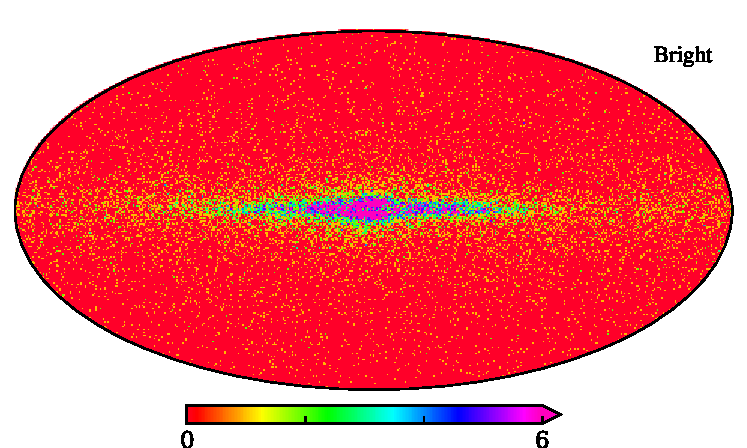
\includegraphics[width=\columnwidth]{figs/sourcecount/source_count.pdf}\\
  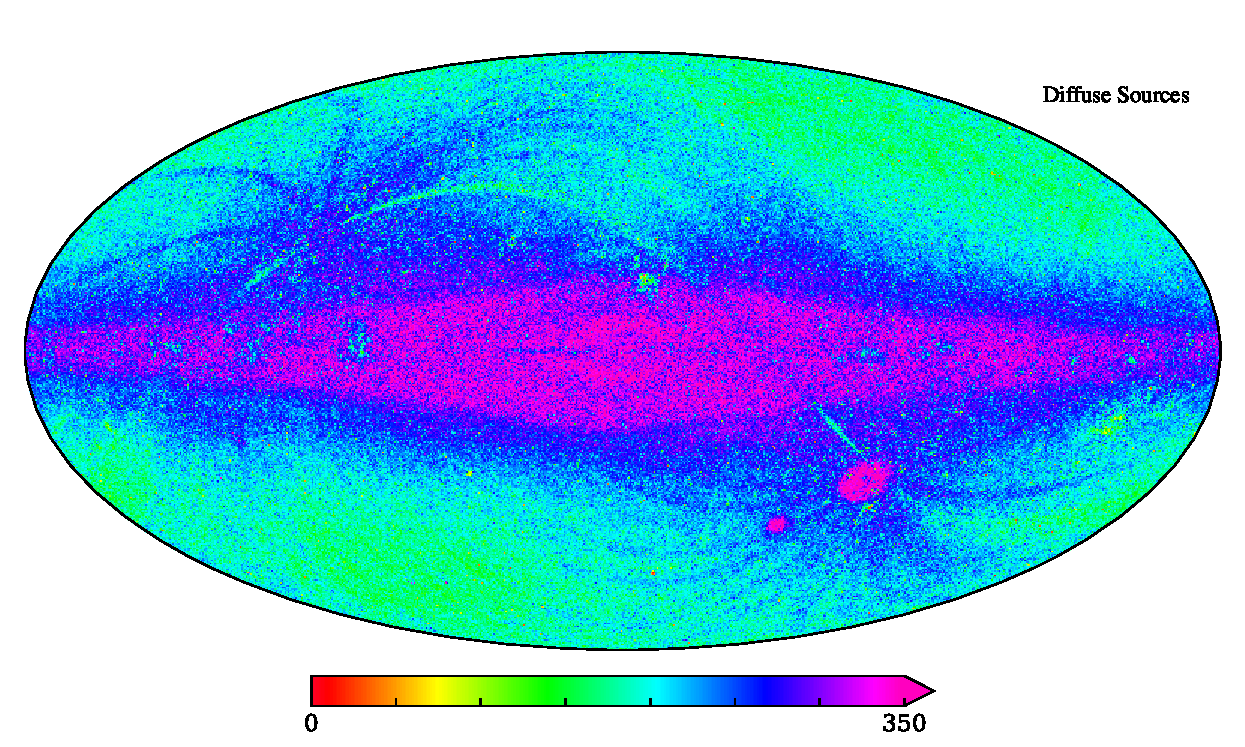
\includegraphics[width=\columnwidth]{figs/sourcecount/diffuse_count.pdf}
  \caption{Top: the total number of bright sources in each pixel, counting both stars and extra sources. Bottom: the total number of sources included in the diffuse template, which shows a clear imprint of the WISE scan strategy.}
  \label{fig:starcount}
\end{figure}

\begin{figure*}
  \centering
  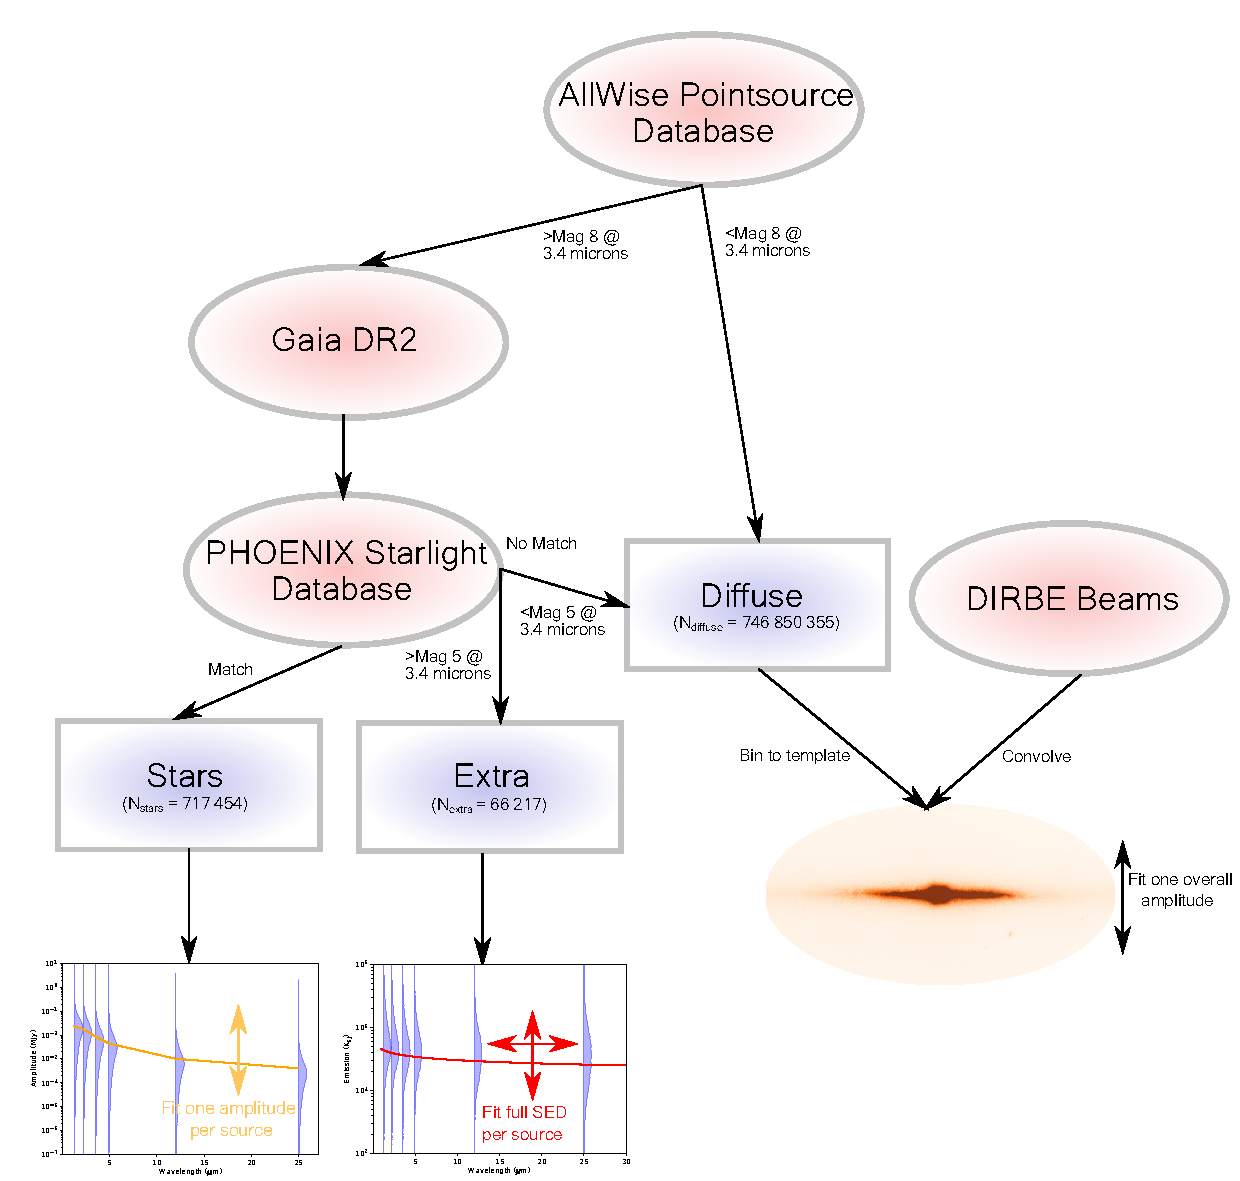
\includegraphics[width=\textwidth]{figs/diagram/dirbe_diagram.pdf}\\
  \caption{Schematic diagram of the commander handling of compact objects in DIRBE. Red ovals are input data, and the blue boxes are the three classes of sources described in this paper. }
  \label{fig:diagram}
\end{figure*}

\subsection{Stars}

\label{sec:starmodel}

For each star we extract estimates of the effective temperature, $T_{\mathrm{eff}}$, the gravitational acceleration, $\log g$, and the metallicity, $[M/H]$, from the GAIA DR2 database \citep{gaiaCat}, and use those to identify a best-fit spectral energy density (SED) from the PHOENIX starlight database \citep{Husser_2013}. The distributions of these parameters for the stars we select are shown in figure \ref{fig:gaiacat}. For stars with $T_{\mathrm{eff}} > 12000$K the PHOENIX catalog lacks data, which means that the 1.1\% of sources with higher temperatures use this 12000K temperature spectra. This could lead to an issue with the SEDs of these hottest stars, but the overall amplitudes are fit per star so this should mitigate the majority of this effect.

\begin{figure}
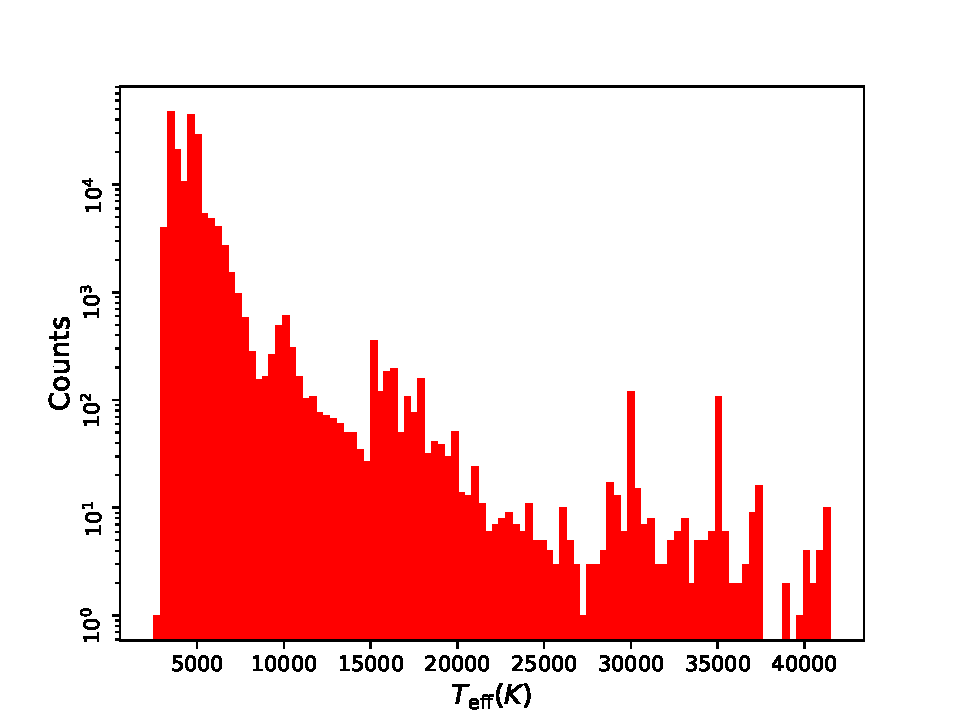
\includegraphics[width=\columnwidth]{figs/gaia/t_eff.pdf}
  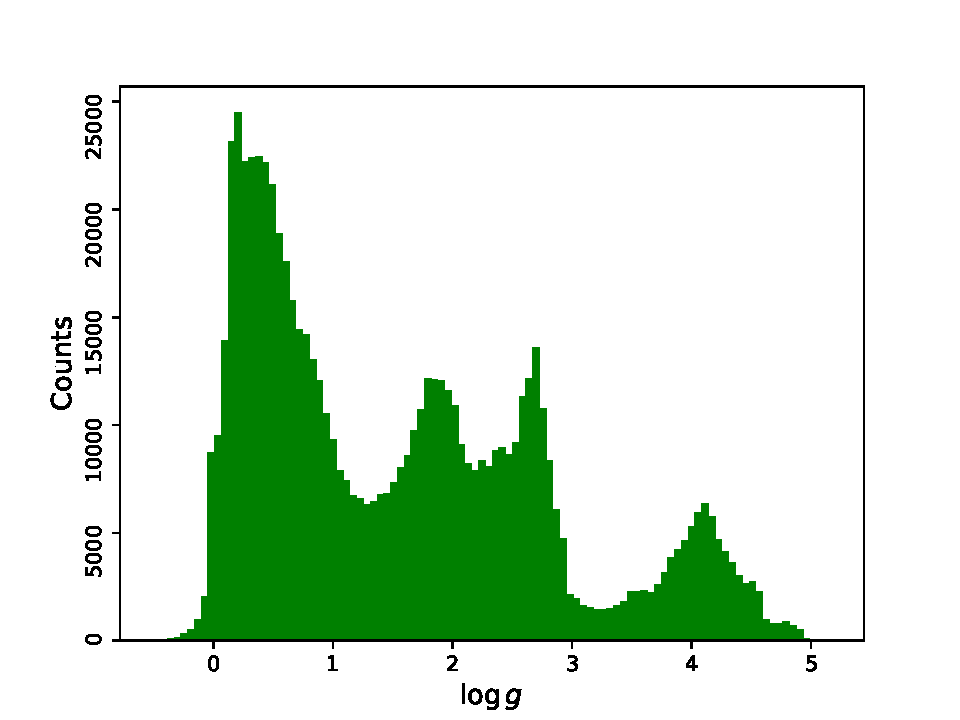
\includegraphics[width=\columnwidth]{figs/gaia/logg.pdf}\\
  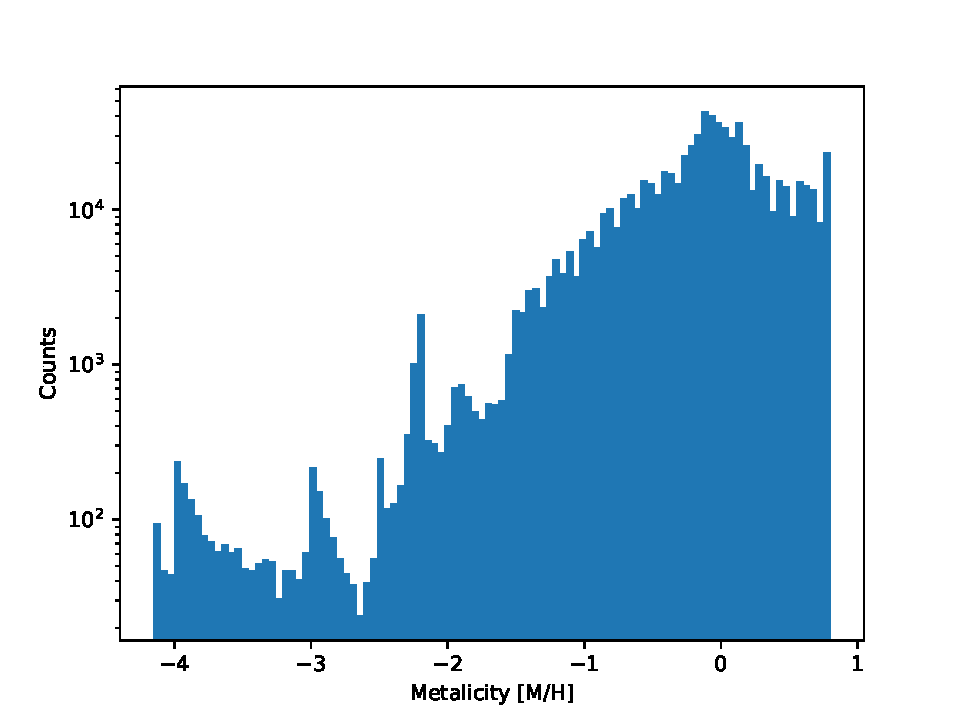
\includegraphics[width=\columnwidth]{figs/gaia/metalicity.pdf}\\
  \caption{Histograms of the three star parameters (effective temperature, gravity and metalicity) that are used by the PHOENIX database to determine the star SEDs, for the 717454 stars used in this analysis.}
  \label{fig:gaiacat}
\end{figure}

The effects of these varying parameters on the star SEDs was examined in figure \ref{fig:catalogueSEDs}. Although these effects are likely well known in the stellar astronomy community, we show them here for cosmologists who do not have an intuition for them. Here, we select a star with $T_{\mathrm{eff}}= 4600$K, $\log g = 3.5$ and $[M/H]= 0.0$ as our reference star, being close to the mean of our sample. We then vary each of the three parameters slightly, holding the others constant and plot difference between the two curves, for both positive variation (top subplots) and negative (bottom subplots). The effective temperature is perhaps not surprisingly the dominant effect on the SED. A simpler model of star parameters in the far-infrared could perhaps neglect $\log g$ and $[M/H]$ entirely and produce SEDs based purely on $T_{\mathrm{eff}}$, and would be nearly as predictive, but we made a conservative choice to include them in the analysis regardless. 

\begin{figure}
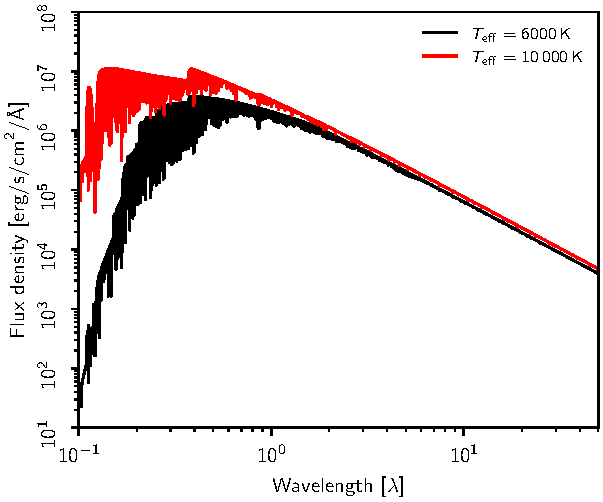
\includegraphics[width=\columnwidth]{figs/gaia/star_SED_Teff.pdf}
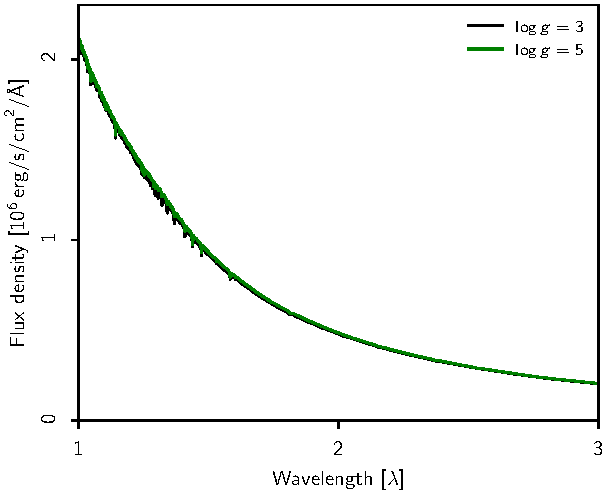
\includegraphics[width=\columnwidth]{figs/gaia/star_SED_logg.pdf}
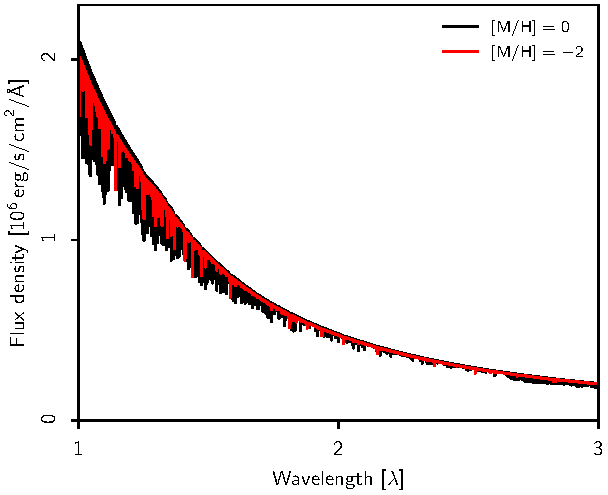
\includegraphics[width=\columnwidth]{figs/gaia/star_SED_MH.pdf}
  \caption{Comparison of PHOENIX spectra for different parameter compbinations. In each panel the black curve shows a reference star spectrum with $T_{\mathrm{eff}}= 6000$K, $\log g = 3.0$ and $[M/H]= 0.0$. The red curve shows, from top to bottom, the resulting spectra when setting $T_\mathrm{eff}=10\,000\,\mathrm{K}$, $\log g = 5.0$, and $[M/H]= -2.0$. The spectra shown in the middle panel have been smoothed to highlight the broad features that are mostly relevant for the current analysis.}
  \label{fig:catalogueSEDs}
\end{figure}

\begin{figure}
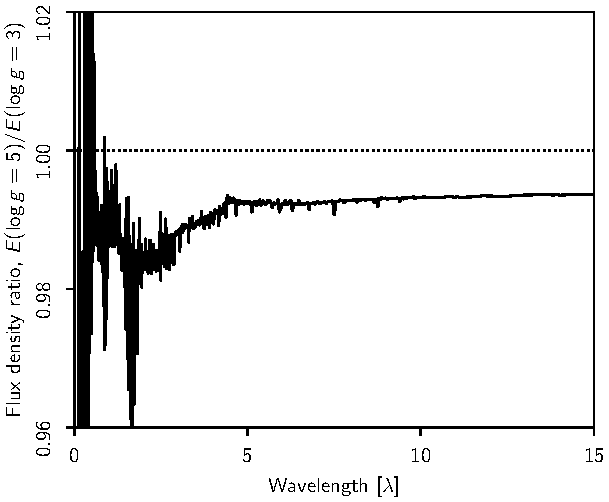
\includegraphics[width=\columnwidth]{figs/gaia/star_SED_logg_ratio.pdf}
\caption{Ratio between the PHOENIX spectra shown in the middle panel of Fig.~\ref{fig:catalogueSEDs}, corresponding to $E(\log g = 5)/E(\log g  = 3)$.}
  \label{fig:logg_ratio}
\end{figure}


The full Bayesian data mode is shown in \cite{CG02_01}, and includes the star component $s_{stars}(p, \lambda_j)$, the star emissions as a function of pixel $p$ and frequency $\lambda_j$ for a band $j$. Equation \ref{eq:datamodel} shows the data model for the star component that we describe in this paper


\begin{equation}
s_{stars}(p, \lambda_j) = \sum_i a_i B_i(p, \lambda_j) E_i(\lambda_j),
\label{eq:datamodel}
\end{equation}

where in the notation of \cite{CG02_01} 

\begin{equation}
f_{\mathrm{GAIA}} = B_i(p, \lambda_j) E_i(\lambda_j),
\end{equation}

which is the beam-convolved SED taken from the PHOENIX catalogue.

Here, we sum over each star $i$, where $a_i$ is a single overall amplitude parameter fit per star and $B_i(p, \lambda)$ is the instrument beam for a detector at frequency $\lambda$ in a pixel $p$ for a given star $i$. $E_i(\lambda)$ is the normalized emission for a given frequency $\lambda$. The emission $E_i$ is drawn directly from the GAIA data and the PHOENIX starlight database, and the beam $B$ is fixed for each detector, so we fit only the overall amplitude $a_i$ for each star in this model. This greatly reduces the degeneracies between the stars and other astrophysical components such as dust, and was found to work better than fitting a full SED per star. We include a star component in DIRBE bands 01-06 (1.25 - 25 $\mu$m), as at longer wavelengths the contribution from star emission was greatly subdominant to zodiacal light and dust, and including that data degraded the quality of the amplitude fits. 

To sample the star amplitudes $a_i$ we attempt to minimize the residual in each band for each source $i$, which can be expressed as a linear minimization problem, analogous to the mapmaking equation

\begin{equation}
\label{eq:minimize}
X_ia_i - Y_i = 0.
\end{equation}

where

\begin{equation}
X_i = S^T N^{-1} S = \sum_{j,p}\frac{E_{ij}^2 B^2_{ij}(p)}{\sigma_j^2(p)} 
\end{equation}

and

\begin{equation}
Y_i = S^TN^{-1}d = \sum_{j,p} \frac{E_{ij}B_{ij}(p) d_j(p)}{\sigma_j^2(p)}.
\end{equation}

Here, $\sigma_j^2(p)$ is the noise in pixel $p$ in band $j$, and $d_j(p)$ is the data map in band $j$ at pixel $p$. To reduce degeneracies, we fit the point sources on a data map with all other astrophysical components already removed, so $d_j(p)$ contains only noise and the point source $i$. The solution to \ref{eq:minimize} is simply $a_i = \frac{Y_i}{X_i}$, which gives a single overall amplitude for each star $i$. To sample the amplitudes, we also include a fluctuation term, such that our final proposal for the amplitudes is given by

\begin{equation}
a_i = \frac{Y_i}{X_i} + \frac{1}{\sqrt{X_i}} N_i(0,1),
\end{equation}

where $N_i(0,1)$ is a sample drawn from a unit Gaussian with 0 mean.

\subsection{Extra Pointsources}

\label{sec:extragalacticmodel}

After fitting the star catalogue, we are left with another background of pointsources, which lack spectral information. Sources that do not match against the GAIA catalogue or that do not have sufficient SED information to model, but which are still brighter than magnitude 5.06 in the WISE $3.4 \mu m$ band ($3000$ MJy) are fit with a more general blackbody of the form:

\begin{equation}
a \frac{e^{\frac{\nu_0 h}{k_b \theta}} - 1}{e^{\frac{\nu h}{k_b \theta}} - 1} * (\frac{\nu}{\nu_0})^{\theta_2 + 1}
\end{equation}

Here, $\nu_0$ is a reference frequency, set to $239833.966$ GHz (1.25 $\mu m$), $\theta_1$ and $\theta_2$ are spectral indexes that describe the source's frequency scaling behaviour, and a is an overall amplitude scaling. 



\subsection{Diffuse Star Emission}

\label{sec:diffusemodel}

Finally, after modelling the brightest sources using one of the two methods described above, we are left with a diffuse background of stars that are too dim to be individually resolved, but that in aggregate form a significant contribution to the total star signal at these wavelengths and so must be accounted for. We model this diffuse background using a single full-sky template, generated from the WISE W1 data at 3.4$\mu$m. We take the full AllWISE pointsource catalog, and select source with a included W1 magnitude that isn't already included in one of the previous pointsource models (ie. sources dimmer than Mag. 8, or less that Mag. 5 with no stellar parameter data). We create a high resolution healpix map \citep{healpix} at nside=2048, and then add each source in turn to this map. We then downgrade the map to nside=512, which gives the map shown in Fig. \ref{fig:diffuse}. 

\begin{figure}
  \centering
  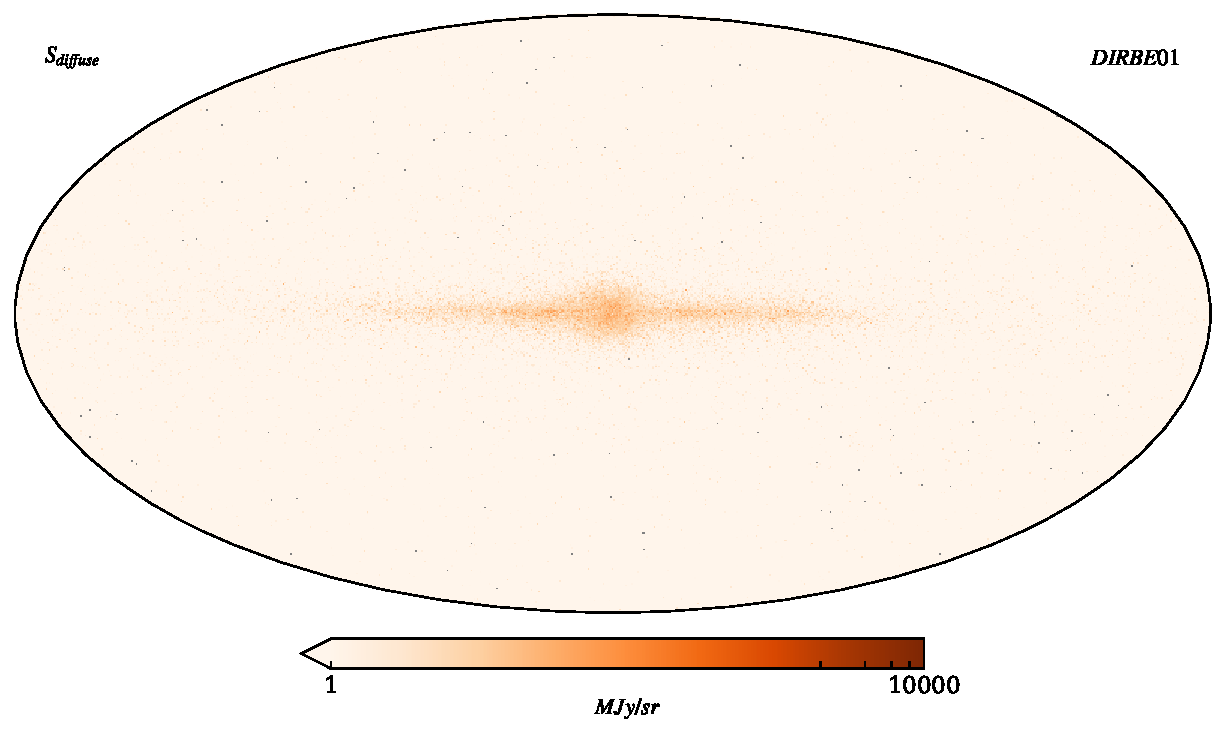
\includegraphics[width=\columnwidth]{figs/diffuseTemplate/diffuse_stars_log.pdf}\\
  \caption{The template of diffuse star emission evaluated in the DIRBE 01 band, plotted on a log scale.}
  \label{fig:diffuse}
\end{figure}

This template is then included in the full sky model, with an amplitude fit jointly in bands 01-04, with an SED given by the mean of all SEDs of all the individual stars modelled in section \ref{sec:starmodel}. This SED is fit with a single amplitude parameter, which compensates for the overall difference in bandpass between W1 and the DIRBE bands. Although bands 5 and 6 do no contribute to the amplitude fit, the template is extrapolated to those bands as well and added to the total sky model.

\section{Astrophysical results}
\label{sec:results}

The model described in the previous section is then included in a full sky model, which includes galactic dust, zodical light and other components. A model of the DIRBE instrument is used to estimate other data artifacts, the most prominent of which was a sun-stationary signal of unknown origins. Following our previous work withing the Cosmoglobe framework \citep{BP01, watts2023_dr1}, we implement this model within the \texttt{commander3} codebase \citep{BP03}, which is our Bayesian end-to-end analysis pipeline. The full posterior of all our model parameters was then sampled using Gibbs sampling, exploring the full space around the maximum likelihood values of each parameter. We computed a total of 810 unique samples spread over 6 independent chains after discarding our burn-in data, which gave robust sample sizes for the results described here. 

In this paper, we present just the results of the star models described in section \ref{sec:models}, but we direct interested readers to the companion papers in the larger data release. More details on the overall sampling approach can be found in \citet{CG02_01}. The other components of the sky model are described in \citet{CG02_02} and \citet{CG02_05}, and our limits on the CIB monopole derived from this work are presented in \citet{CG02_03}. 


\subsection{Maps}

In Figure \ref{fig:starsT} we show the mean compact object maps for the full pipeline run in all six DIRBE bands where they are modelled. Here, the maps show the sum of star component, the extra source component, and the diffuse background, which fully accounts for the pointsource emission over the full sky. As expected, the majority of the emission is found in the galactic plane, but there is also an important contribution from high latitude stars.

\begin{figure*}
  \centering
  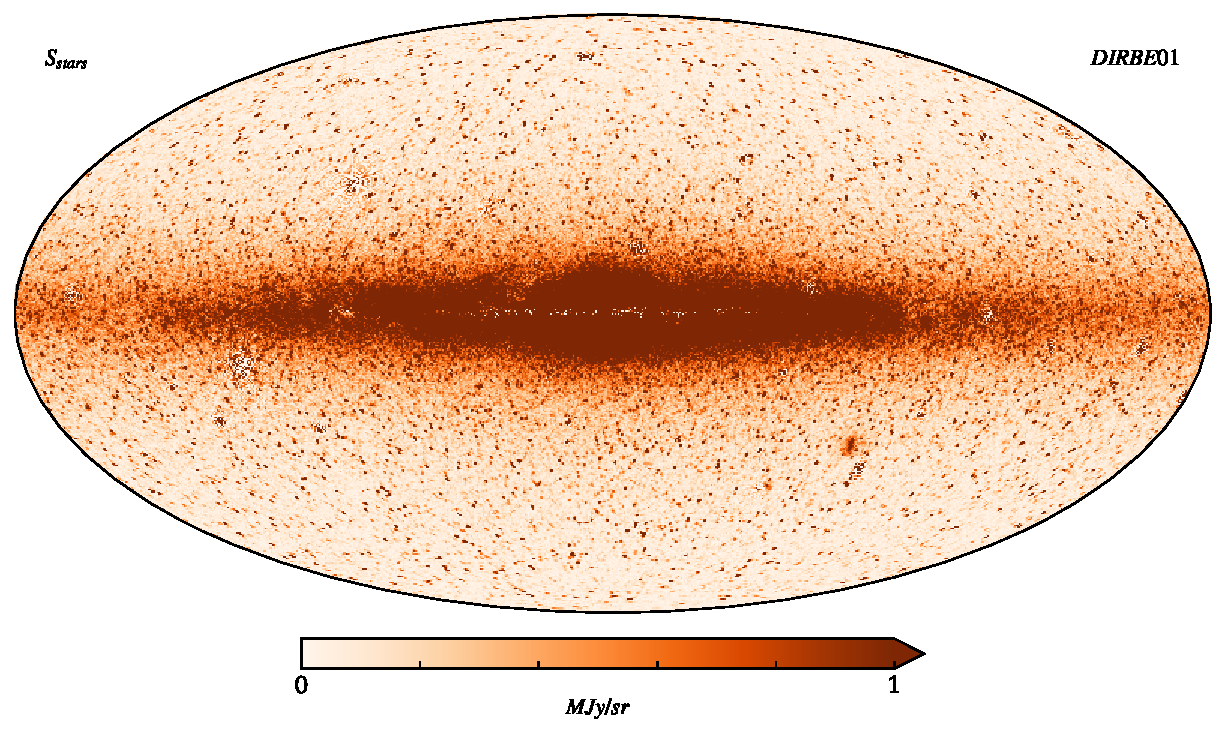
\includegraphics[width=0.49\textwidth]{figs/starmaps/all_stars_mean_01.pdf}
  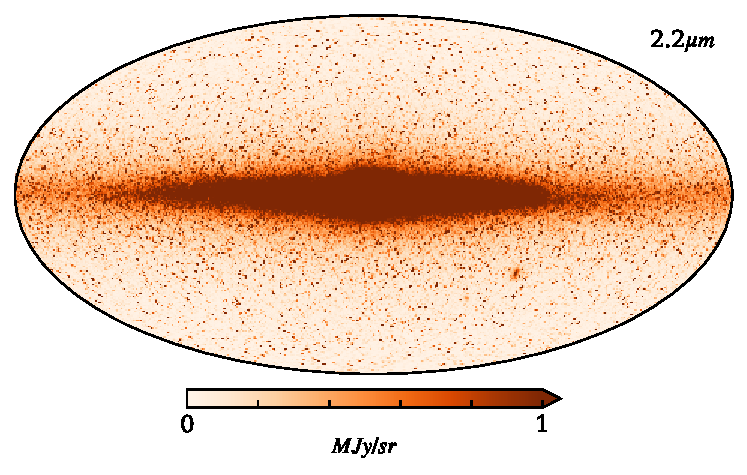
\includegraphics[width=0.49\textwidth]{figs/starmaps/all_stars_mean_02.pdf} \\
  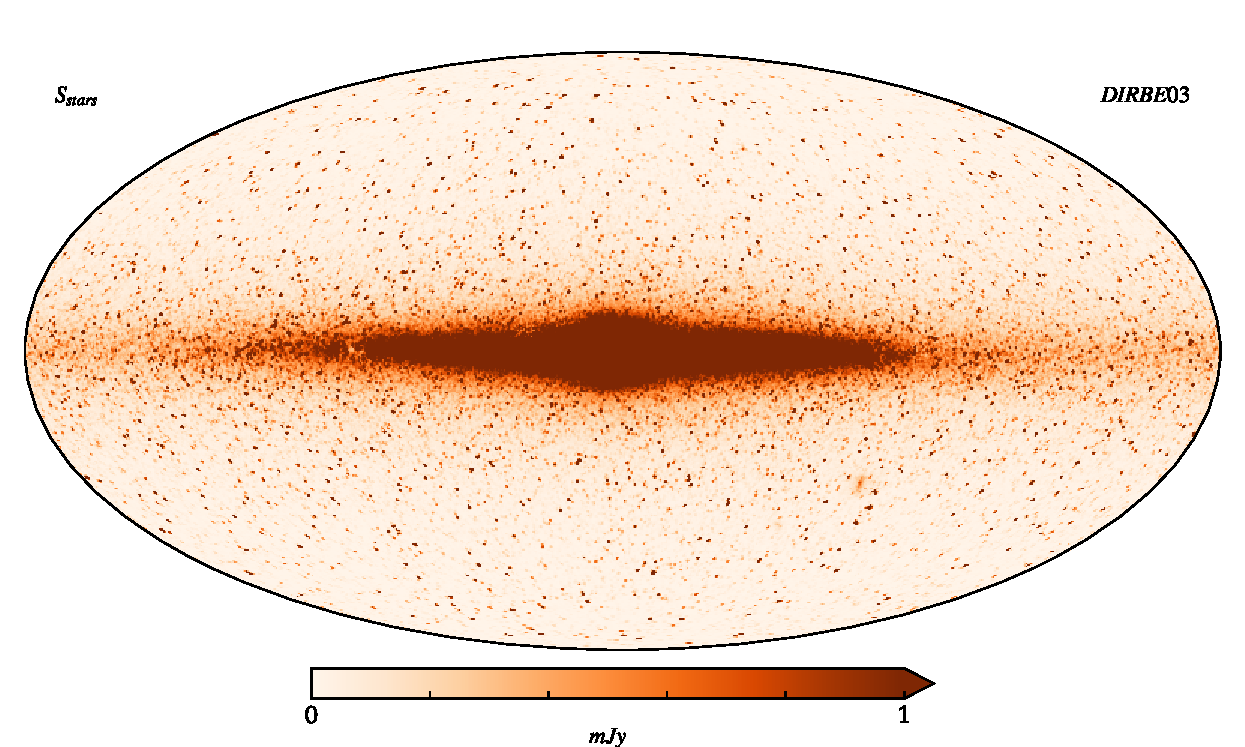
\includegraphics[width=0.49\textwidth]{figs/starmaps/all_stars_mean_03.pdf}
  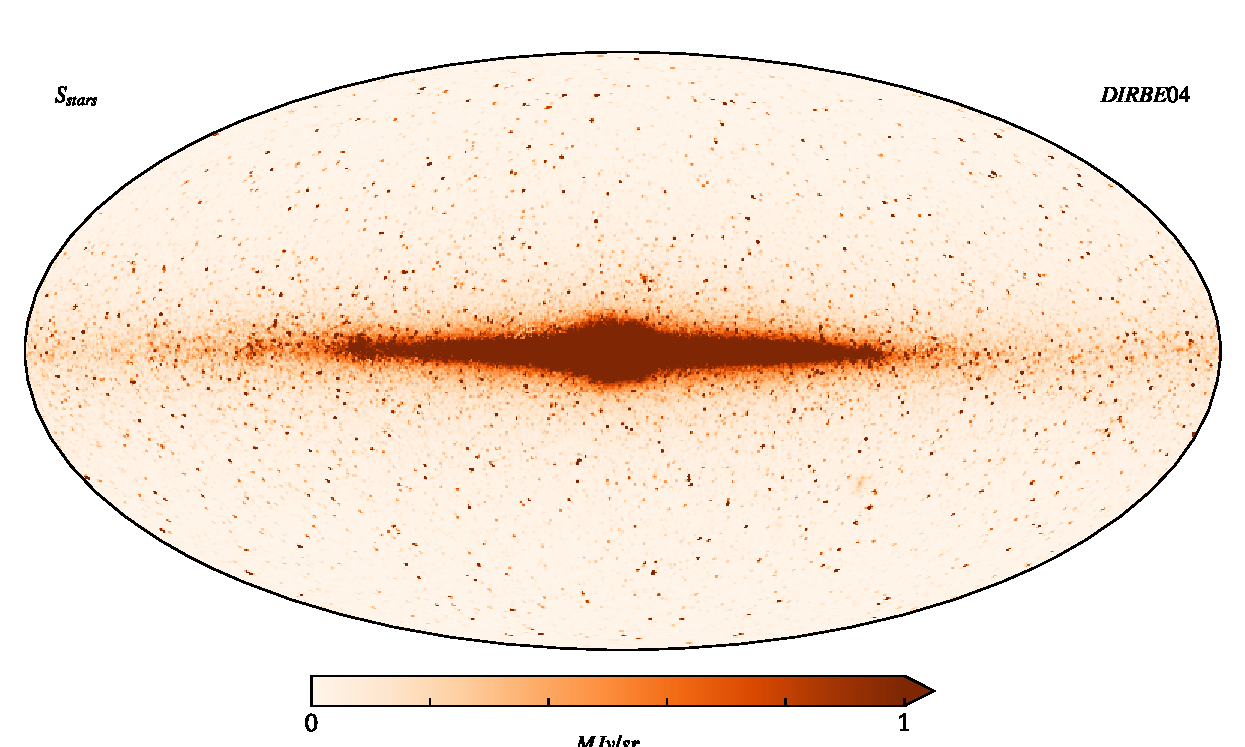
\includegraphics[width=0.49\textwidth]{figs/starmaps/all_stars_mean_04.pdf} \\
  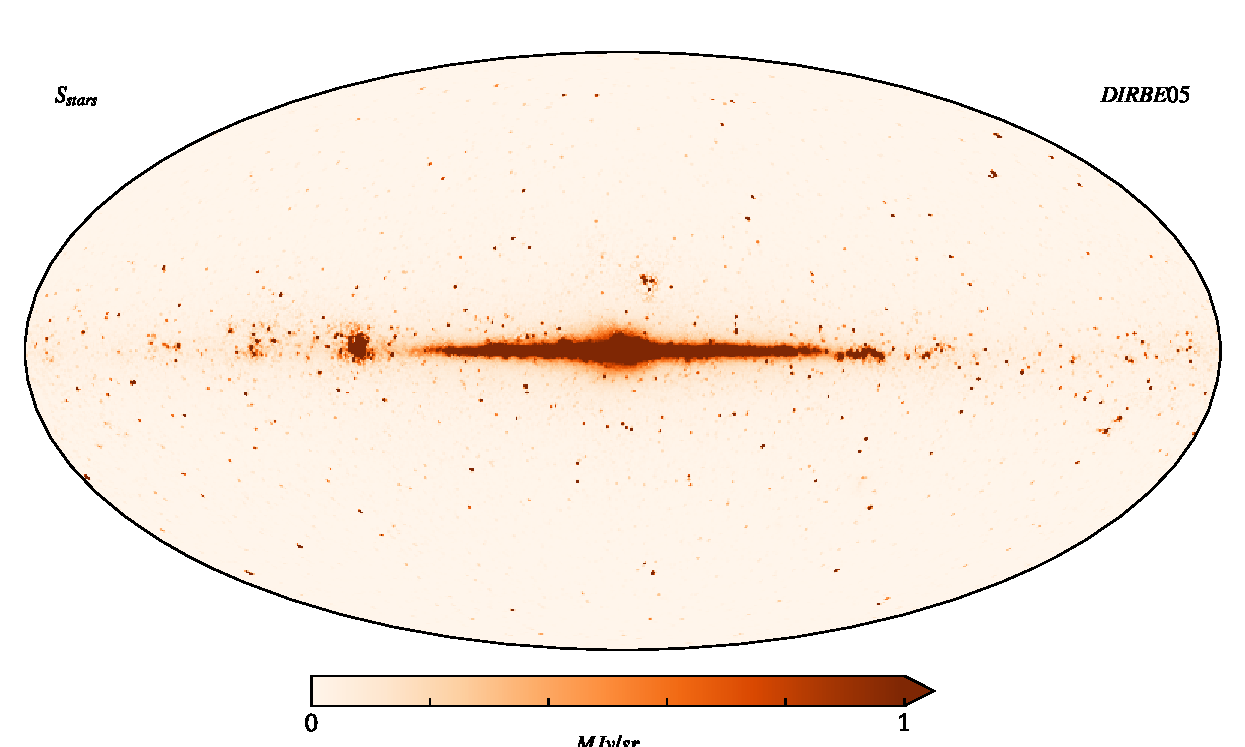
\includegraphics[width=0.49\textwidth]{figs/starmaps/all_stars_mean_05.pdf}
  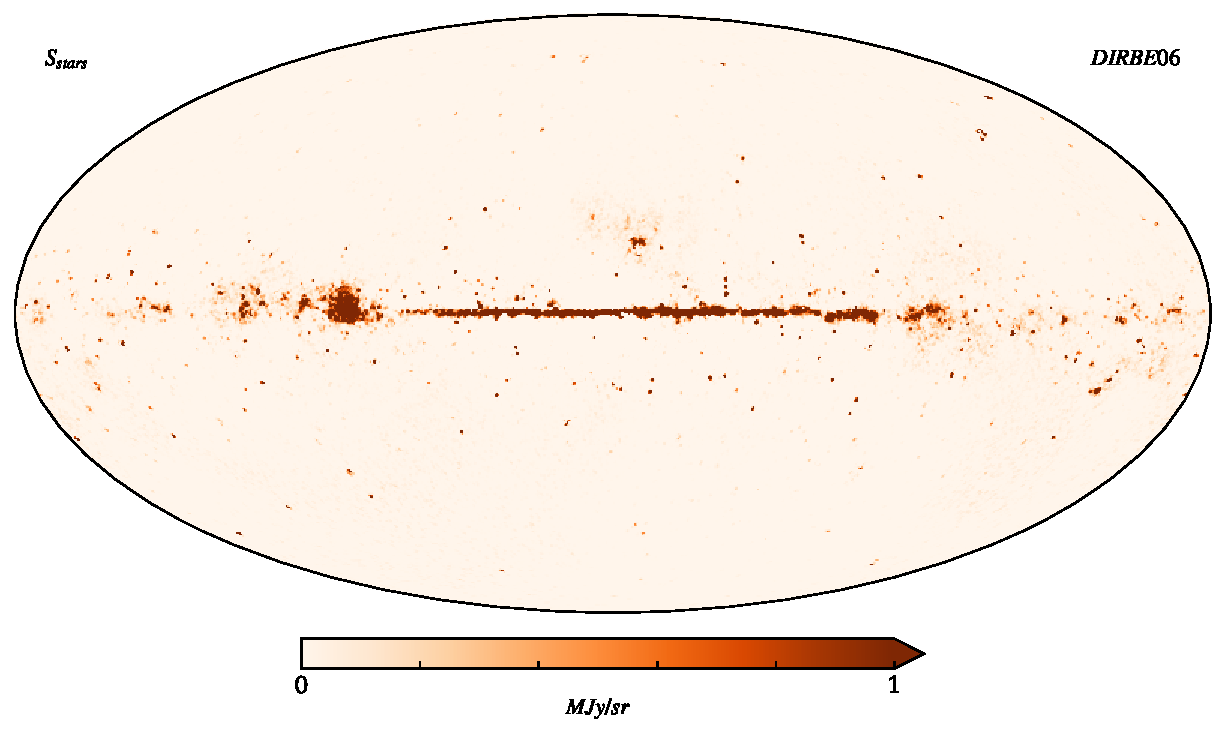
\includegraphics[width=0.49\textwidth]{figs/starmaps/all_stars_mean_06.pdf} \\
  \caption{Mean compact object maps from the Cosmoglobe DR2 release for the first 6 DIRBE bands. }
  \label{fig:starsT}
\end{figure*}

In Figure \ref{fig:zooms} we show zoom ins of a 20$^\mathrm{o}$ patch of sky centered at (lon, lat)= $20^\mathrm{o}, 70^\mathrm{o}$, plotting the DIRBE sky map in each band for the four highest frequency bands where the stars are most significant. In the second column, we show the total star model for the same region, and then the resulting residual after removing the sky model from the data. The residuals contain a variety of mis-modeled point sources, as well as noise, and hints of cosmic structure like the CIB \citep{CG02_03}. 

We can identify three types of pointsource residuals in this third column, although there are a large number of sources with residuals that are subdominant to the background noise level and so can be considered to be well modelled. Some of the pointsources clearly show the imprints of spectral complexity, where the residual signature is blue in some bands and red in some others, which implies that our knowledge of the spectra is imperfect and a single overall amplitude fit was insufficient to model that source. The second class of residuals appear to be ring shapes, where the center of the pointsource is modelled well, but we oversubtract emission around the edges. This could be caused by our simplistic modelling of the DIRBE beams, which relies on the scanning strategy to symmeterize the otherwise square beam profile of the DIRBE instrument.

Other pointsource residuals are more complex, and look to be superpositions of multiple sources in the same region. These residuals could possibly be reduced by pruning pointsources from the model that are too close to one another, or potentially by improving our models of the brightest sources. No attempt to do so was made in this work, as these residuals were only a small fraction of the total sky, and can be handled by masking if necessary.

\begin{figure*}
  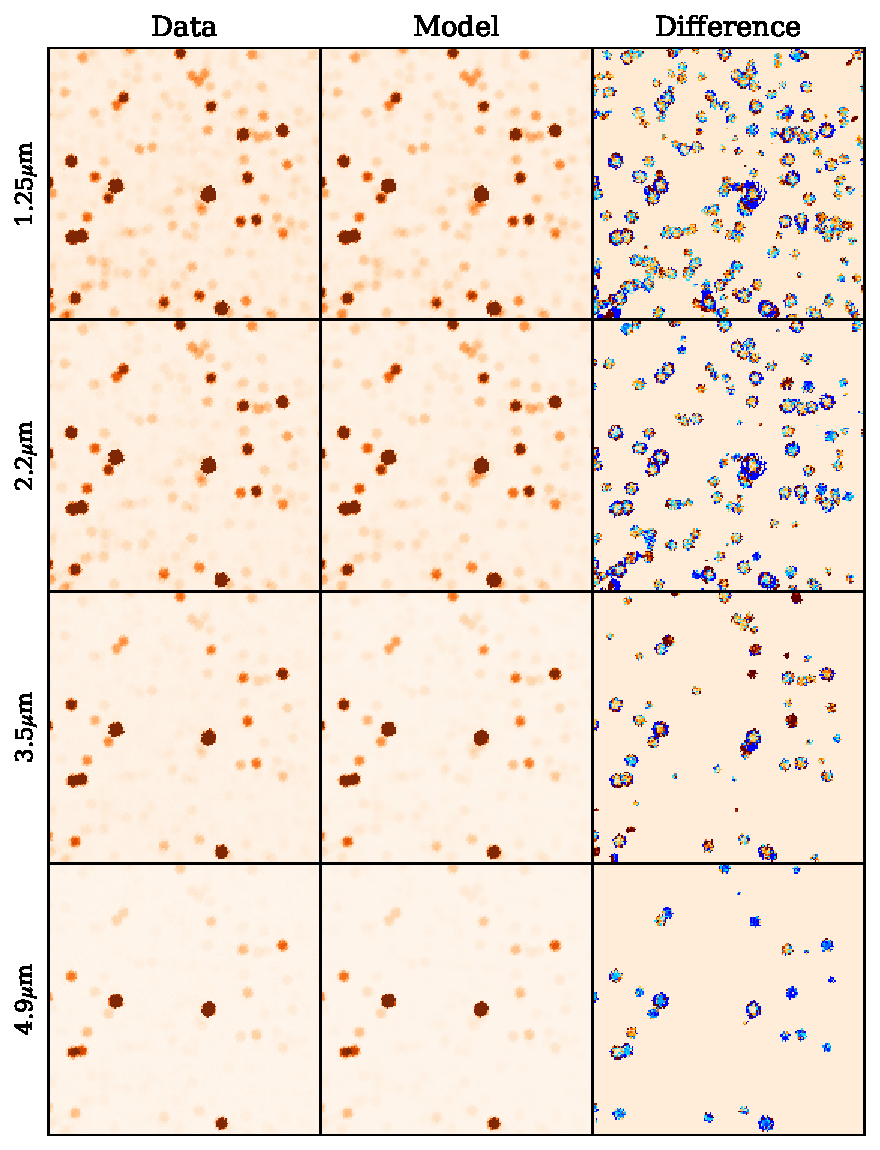
\includegraphics[width=0.95\textwidth]{figs/zoom/combined_zoom.pdf}\\
  \vspace{-8pt}
  \hspace{1.5in}
  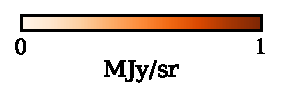
\includegraphics[scale=1]{figs/zoom/cbar1.pdf}
  \hspace{1.1in}
  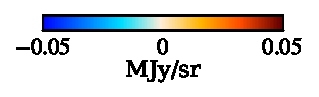
\includegraphics[scale=1]{figs/zoom/cbar2.pdf}
  \caption{Zoom-ins on a subregion of the sky centred at $(20^\mathrm{o},70^\mathrm{o})$. }
  \label{fig:zooms}
\end{figure*}


In Figure \ref{fig:amptrace}, we show the total amplitude of the compact sources in three pixels in different regions in the sky as a function of iteration, for each of our six independent sampling chains. The first 25 samples in each chain are discarded as burn in, and the remaining samples (810 in total) form the samples included our analysis. We see good mixing of the total amplitudes in the top row, although examining the individual components we do see degeneracies.
Especially in the galactic plane, the bottom rows show that the three classes of emissions are trading off between each other (see for example the red chain around sample 115 in the first column). This degeneracy is not unexpected, as the model contained many pixels with more free parameters than data measurements. The fact that we see good mixing in the summed amplitudes, however, gives us confidence that the total model is robust despite this type of internal degeneracy.

\begin{figure*}
  \centering
  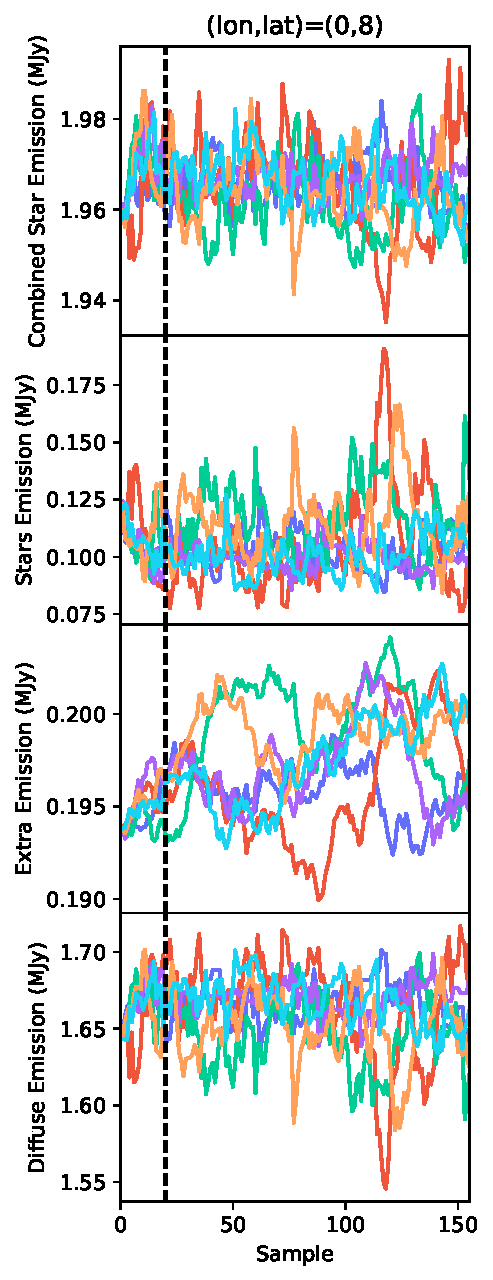
\includegraphics[width=0.32\textwidth]{figs/mixing/trace_1352704.pdf} 
  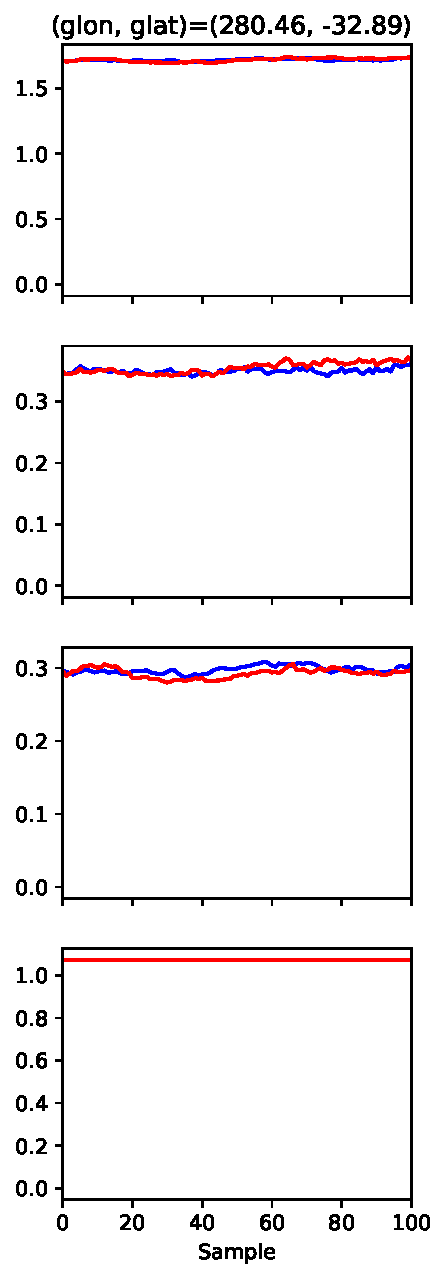
\includegraphics[width=0.31\textwidth]{figs/mixing/trace_2429499.pdf}
  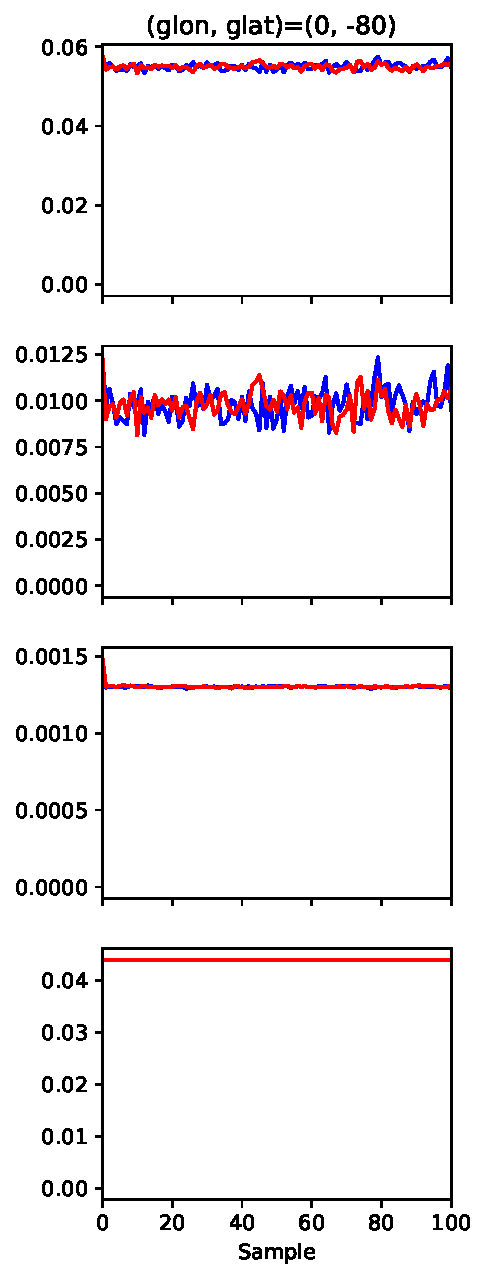
\includegraphics[width=0.326\textwidth]{figs/mixing/trace_3121308.pdf}\\
  \caption{Trace plots of the total star amplitude in all six chains for three pixels in different regions of the sky (low latitudes, the LMC and high latitudes) in DIRBE band 01. The dashed vertical line indicates the end of the burn in period, and samples after that are included in our final sample set.}
  \label{fig:amptrace}
\end{figure*}

\begin{figure*}
  \centering
  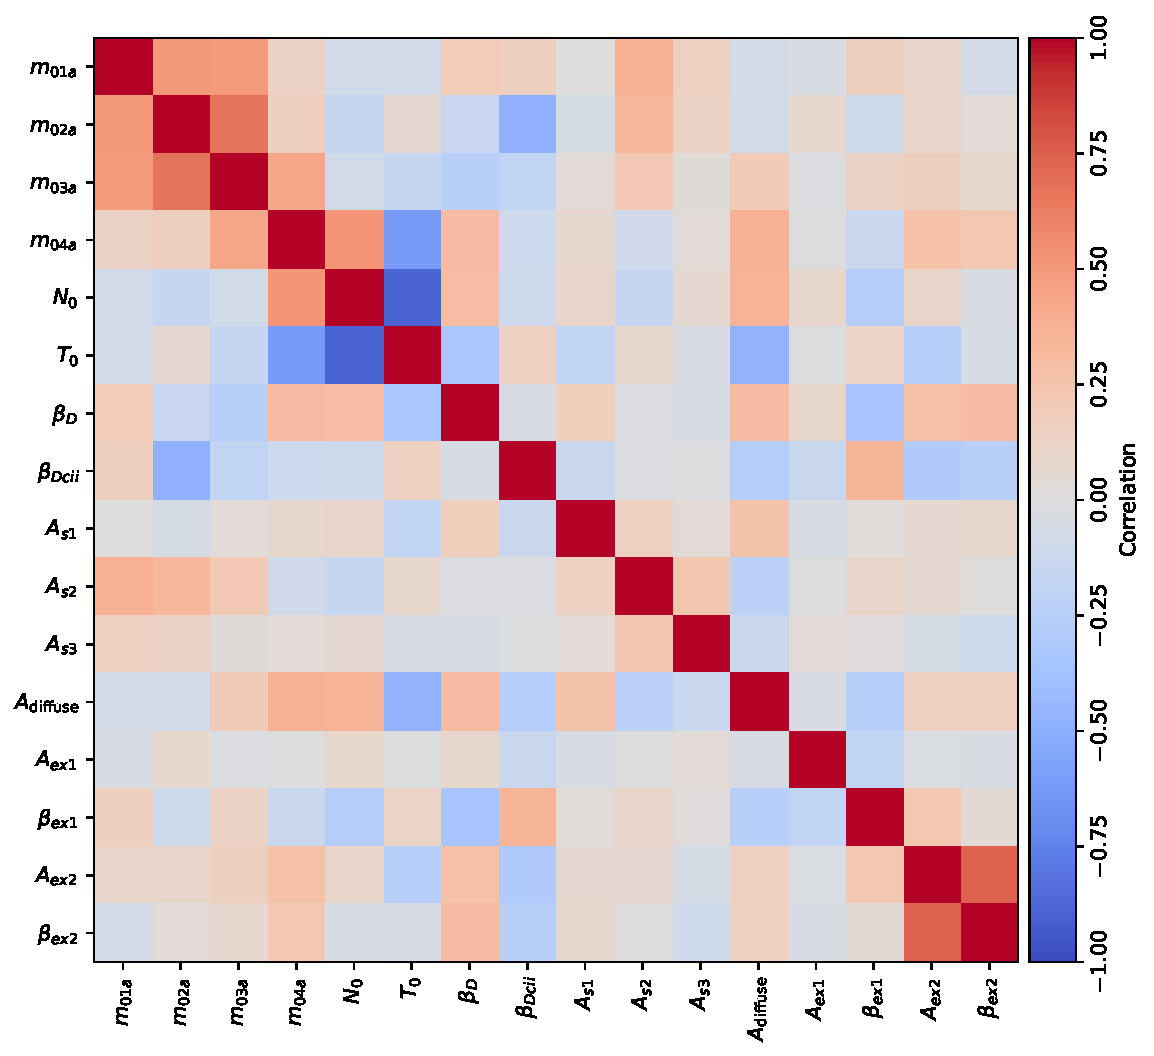
\includegraphics[width=\textwidth]{figs/correlation/covmatrix.pdf}
  \caption{Correlation plot showing a selection of parameters relevant for star modelling. From top to bottom: the monopoles for DIRBE channels 01-04, $N_{0}$ and $T_0$, the full sky ZL parameters, dust beta for the dust and cii correlated dust components, the amplitudes of three randomly selected stars, the diffuse template amplitude and the amplitudes and spectral indexes for two randomly selected extragalactic sources.}
  \label{fig:corr}
\end{figure*}

Figure \ref{fig:corr} shows the correlation matrix, computed between each parameter over all 810 samples. In this case, we include a sample of star parameters, as well as some other parameters where we suspect degeneracies may occur. We see correlations between the monopoles of the 01, 02 and 03 bands, and anti correlations between some of the zodiacal light parameters, as has been studied in \citep{CG02_01, CG02_02}, but no correlations between these and the star model parameters, implying that they are independent. We do see correlation between the spectral and amplitude parameters of the randomly selected extragalactic sources ex$_1$ and ex$_2$, which is likely due to weak constraining power on these objects with only a few bands. These sorts of internal degeneracies within the star parameters are what drove our adoption of the simple "star" modelling approach with a single amplitude per source, and so it is not unexpected that the extra pointsources that are fit without the benefit of spectral information from Gaia show this behaviour still. We do not see much cross correlation between the star parameters and other parameters in the global chain, which implies that the star parameters are well mixed and are not degenerate with other full sky parameters in the run.

\subsection{Spectral Energy Densities}

In addition to the amplitude maps at each frequency, we can also examine the spectra energy densities (SEDs) of the sources within our model. Figure \ref{fig:starSEDs} shows the SED models for all 717454 star sources in our catalogue, as well as the full sky mean SED, which is used as the SED for the diffuse template component. 

\begin{figure}
  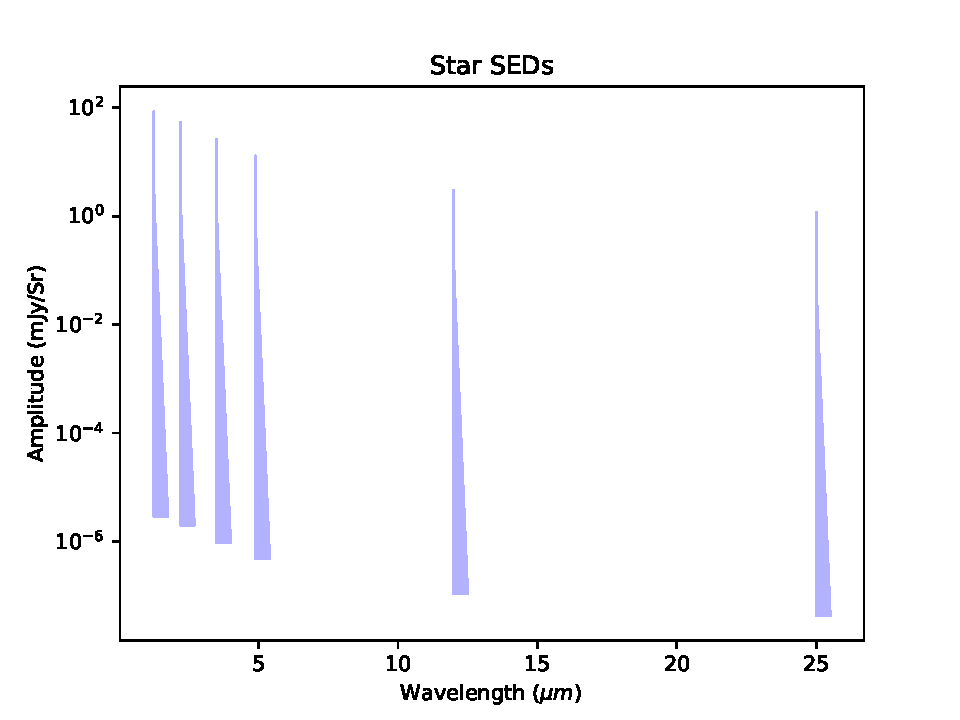
\includegraphics[width=\columnwidth]{figs/starseds/star_seds.pdf}
  \caption{Star emission as a function of wavelength. In blue we have the distributions of amplitudes for each source in our catalogue as a function of frequency. Each star has a fixed SED that is fit with a single amplitude parameter, and after this fitting process we obtain the distributions shown here at each frequency. Overplotted in orange is the mean of these distributions, which is used as the SED for the diffuse template.}
  \label{fig:starSEDs}
\end{figure}

\begin{figure}
  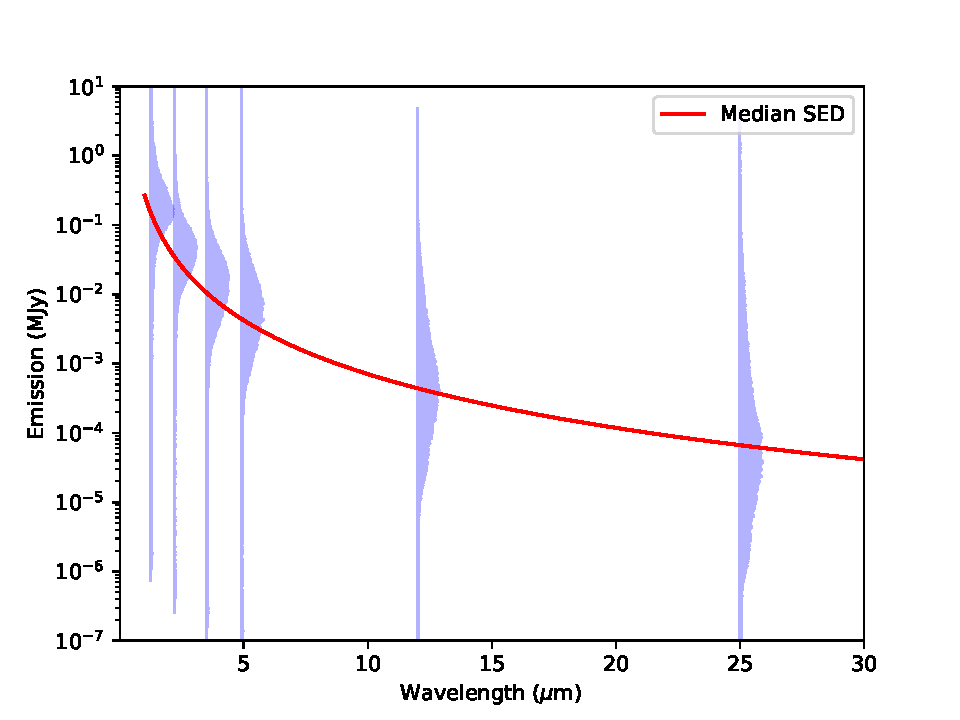
\includegraphics[width=\columnwidth]{figs/starseds/exgal_spectra.pdf}
  \caption{Distribution of extra source spectra as a function of wavelength, shown for the highest frequency DIRBE bands. Overplotted in red is the median source from the ensemble. TODO: convert to mjy/sr}
  \label{fig:exgalSEDs}
\end{figure}

Figure \ref{fig:exgalSEDs} shows the spectra for the extra sources in the same format as fig. \ref{fig:starSEDs}, with the median SED highlighted in red. Overall, we see similar spectral behaviour between these two classes of sources, despite the different modelling approaches. This implies that they may be similar populations of sources (see sec. \ref{sec:extragalactic?}). The extra sources are on average brighter, due to the larger magnitude cuttoff when selecting these sources (dimmer ones were incorporated into the diffuse template). Both classes of sources follow a roughly gaussian amplitude distribution at each frequency, showing no signs of a sharp cuttoff caused by our amplitude cut during the selection process. This is likely due to degeneracies between nearby sources in the model. Those with low amplitudes have had some of their emission sucked up by a nearby brighter source, possibly one within the same $0.11^{\mathrm{o}}$ pixel. About 46\% of sources end up with amplitudes consistent with 0, and are not shown in these plots and so in a subsequent analysis these sources could be trimmed from the model to save computational time and reduce its complexity.


\section{Comparison to other Analyses}
\label{sec:consistency}

\subsection{DIRBE FSM}

The original DIRBE analysis team \citep{dirbeFaint} also removed point sources from their measurement of the CIB emission, but followed a different approach. Instead of modelling the bright sources, the original analysis simply masked pixels brighter than a threshold (15 Jy in band 01), which resulted in cutting almost 35 \% of the sky at 1.25 $\mu$m. For the diffuse sources, they build a model (the "faint source model" or FSM) using the mechanism of \cite{wainscoat}, which integrates a model of source counts over the full sky, including models of galactic morphology, 87 discrete source types and the contribution from dust extinction. The results of this model in the DIRBE 01 band are shown in Figure \ref{fig:DIRBEfaint}, as well a comparison of the two models. 

The top two panels of Figure \ref{fig:DIRBEfaint} shows our diffuse template and the FSM, converted from QuadCube to healpix and plotted at nside=256. The third image shows the difference between these two templates of star emission, which clearly shows a difference in the treatment of dust extinction in the galactic plane. At 1.25$\mu$m, we can clearly see evidence of extinction in the DIRBE data, as can be seen in the fourth panel of fig. \ref{fig:DIRBEfaint}, and so the fact that our model predicts none compared to the FSM is a clear shortcoming. 

\begin{figure}
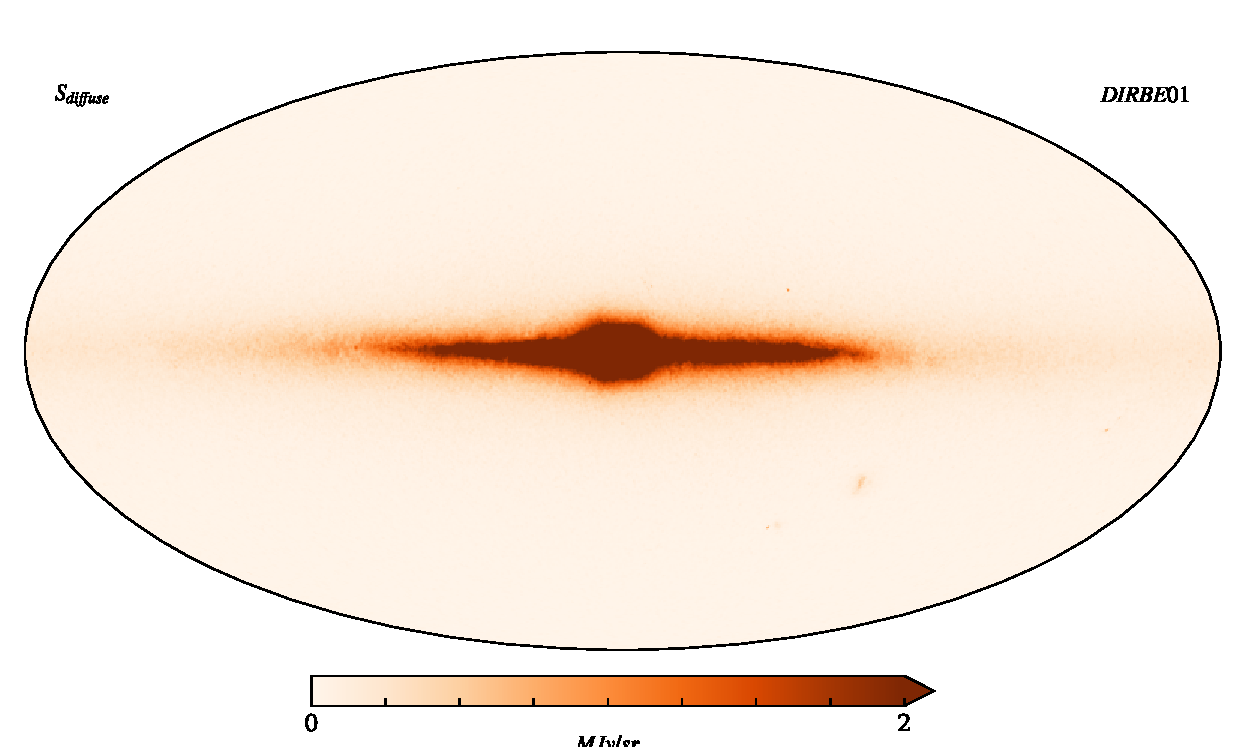
\includegraphics[width=0.9\columnwidth]{figs/diffuseTemplate/diffuse_stars.pdf}  \vspace{-4pt}\\
  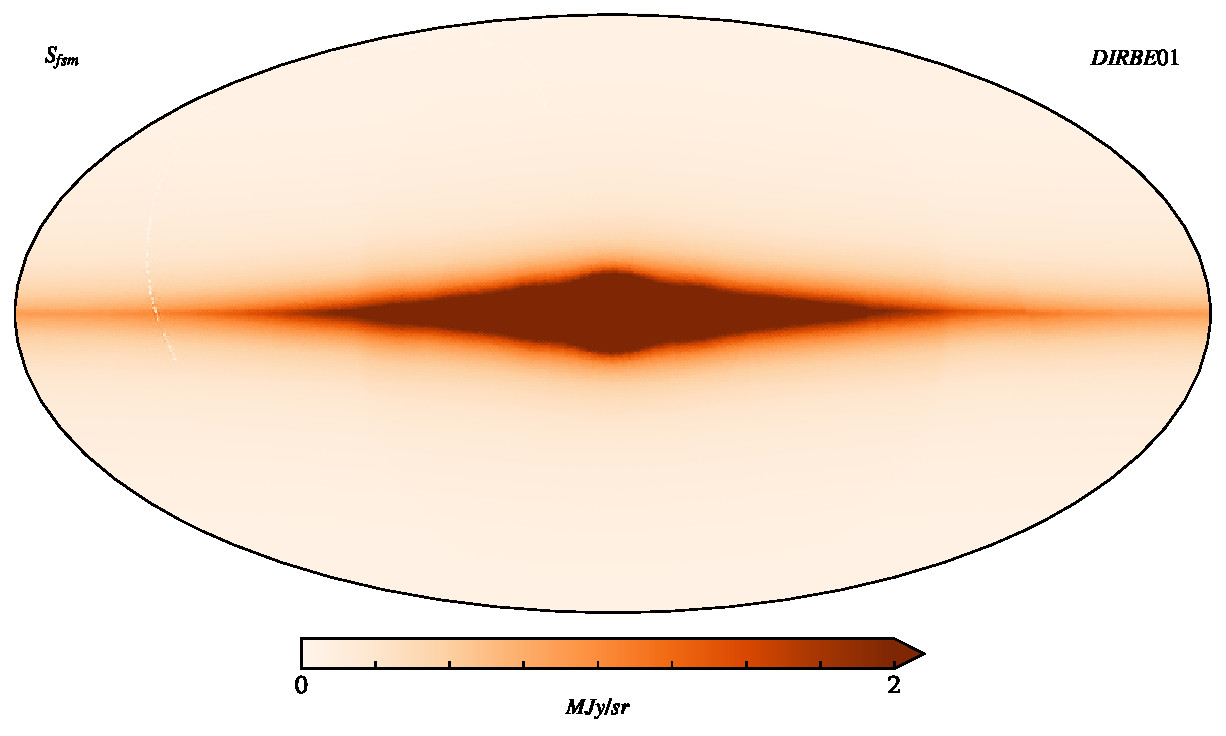
\includegraphics[width=0.9\columnwidth]{figs/diffuseTemplate/dirbe_template.pdf}\\
  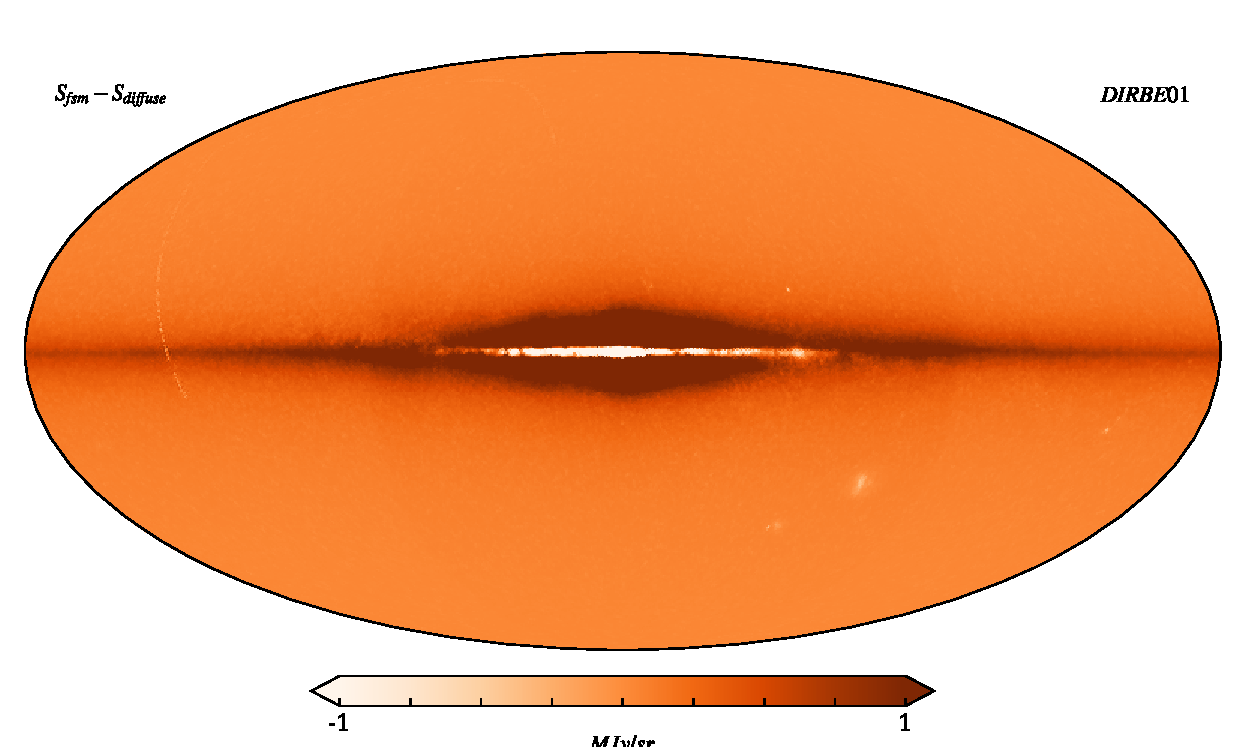
\includegraphics[width=0.9\columnwidth]{figs/diffuseTemplate/diffuse_diff.pdf}\\
  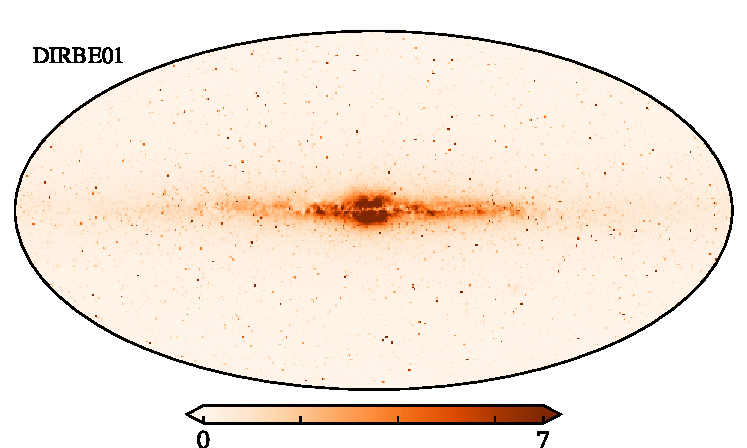
\includegraphics[width=0.9\columnwidth]{figs/diffuseTemplate/band_01_map.pdf}\\
  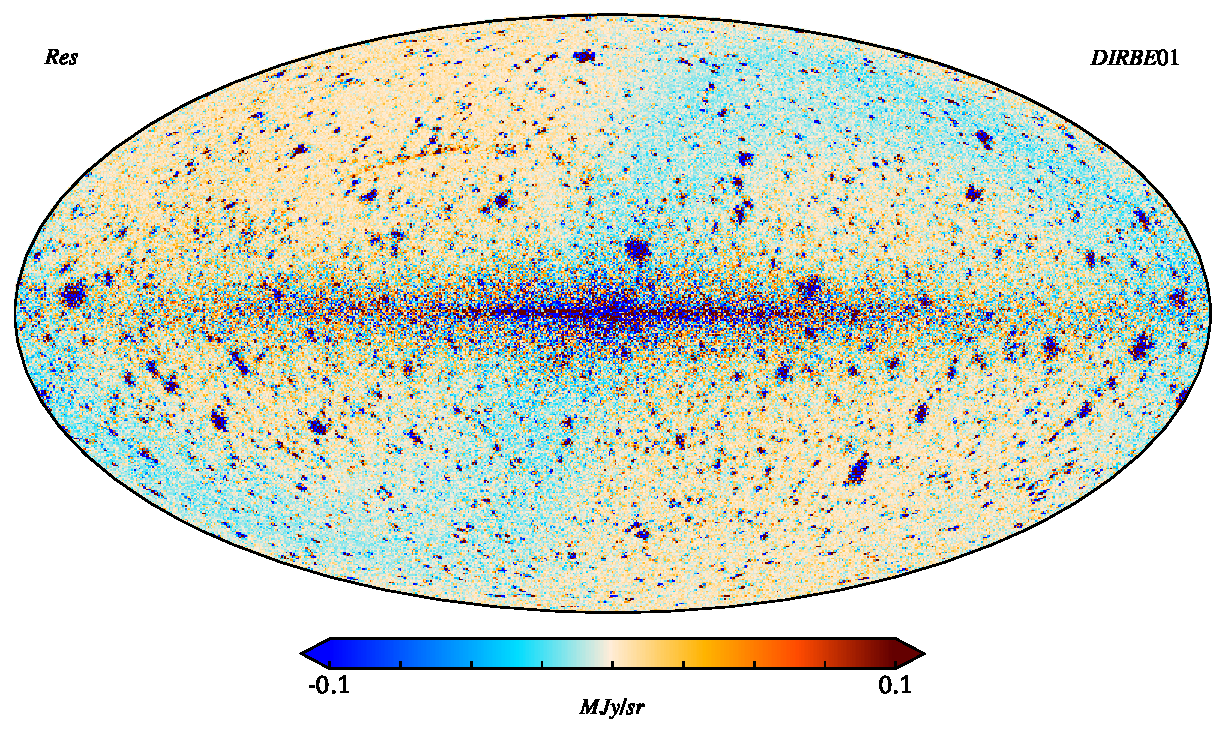
\includegraphics[width=0.9\columnwidth]{figs/diffuseTemplate/band01_res.pdf}\\
  \caption{The Commander diffuse star template (Top). Next: The DIRBE faint star model at 1.25 $\mu$m retrieved from LAMBDA and converted from QuadCube to healpix and the difference between that model and the diffuse template (position 3). The fourth panel shows our zodi-subtracted frequency map for the DIRBE 01 band, and the bottom panel shows the DIRBE 01 residual from the Commander run, indicating that our star model is slightly overestimating signal in the galactic plane, possibly due to missing extinction.}
  \label{fig:DIRBEfaint}
\end{figure}

This difference shows that our model based on the integrated AllWISE pointsource catalogue predicts more star emission in the galactic plane than the DIRBE FSM in the inner part of the plane where dust extinction is dominant. This is likely due to the model being produced based on star emissions measured at 3.4$\mu$m, which shows less relative extinction than the data at 1.25$\mu$m. 

In the galactic bulge, our model predicts less emission than the FSM, which, when we look at the bottom panel of fig. \ref{fig:DIRBEfaint}, seems to be a better fit to the data. The blue residuals in the galactic center show that the model overpredicts emission in general in the galaxy, so  increasing the emission to the level that the FSM predicts would be a worse fit in this region. 

\begin{figure}
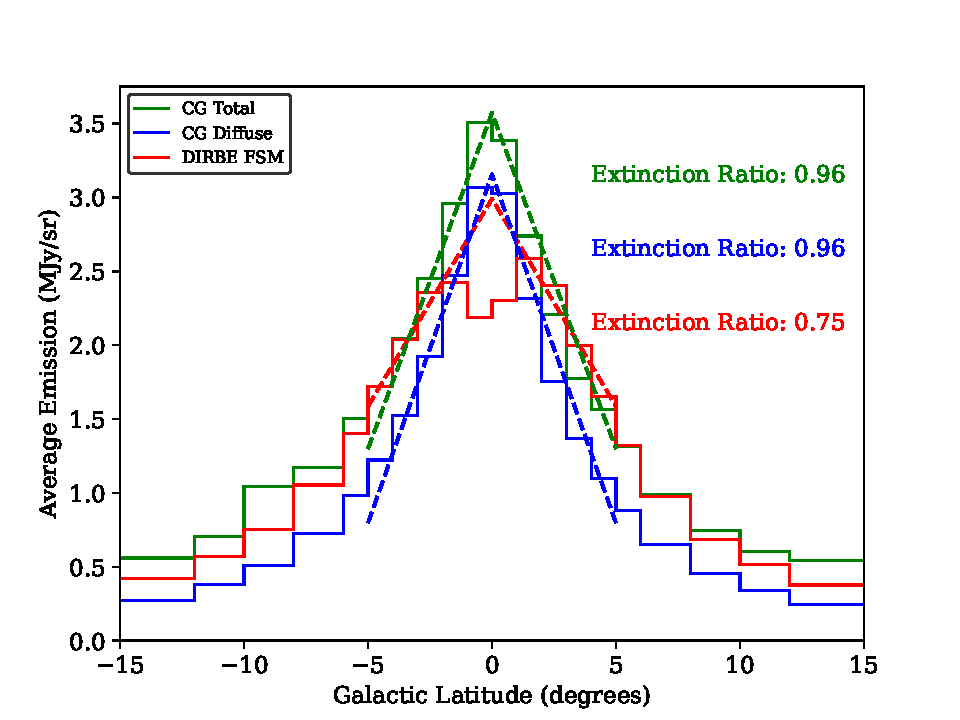
\includegraphics[width=\columnwidth]{figs/diffuseTemplate/extinction.pdf}
  \caption{Profiles of the DIRBE Faint Star Model (FSM) and Diffuse template as a function of galactic latitude. A linear extrapolation is overplotted in the core region from -5 to 5 degrees galactic latitude, but excluding the galactic center from -1 to 1 degree. The theoretical value central value from this fit is compared to the measured values in the central bins to give estimates of the dust extinction in the galactic center for both cases.}
  \label{fig:extinction}
\end{figure}

Figure \ref{fig:extinction} shows another comparison of these two models, highlighting mean behaviour as a function of galactic latitude which shows this missing extinction clearly. The DIRBE FSM shows clear dust extinction in the galactic center at 1.25 $\mu$m, as it explicitly incorporates extinction estimates from the 100 $\mu$m band, whereas the cosmoglobe model built from the Gaia data doesn't show significant extinction on this plot. Regardless, it is surprising to not see any evidence of extinction in the galactic center as previous estimates such as \cite{extinction} estimate it at 70\% at 1 $\mu$m and 94\% at 3.4 $\mu$m. \emph{HK: Is this the case? I am confused by table 3 in rieke+lebofsky. Are they showing just the total scaling of the emissions, or is it actually a measure of the relative extinction in dusty regions?}

\subsection{DIRBE and 2MASS}

After the official DIRBE analysis, \cite{DIRBE2mass}, following \cite{gorjian} used the 2MASS catalogue to remove star emissions from DIRBE and find an improved upper limit on the CIB monopole, but were ultimately unable to claim a detection due to the zodiacal light contamination that they were could not correct. Their analysis looked at four dark patches of the sky and used 2MASS to estimate the contribution of both bright (K band magnitude > 14) and faint sources to the total signal in each patch, which we can compare with the Cosmoglobe estimates, as shown in Table \ref{tab:2mass}.

\begin{table*}
    \centering
    \newcolumntype{C}{ @{}>{${}}r<{{}$}@{} }
    \begin{tabular}{l c c c c c c c c c}
    \hline
    \hline
     Patch & $l$ & $b$ & $r$ & \multicolumn{2}{c}{Bright Stars} & \multicolumn{2}{c}{Diffuse Stars} & \multicolumn{2}{c}{Sum}\\ 
     & ($^{\circ}$) & ($^{\circ}$) & ($^{\circ}$) & \multicolumn{2}{c}{(kJy/sr)} & \multicolumn{2}{c}{(kJy/sr)} & \multicolumn{2}{c}{(kJy/sr)}\\
          &  & & & \cite{DIRBE2mass} & CG & \cite{DIRBE2mass} & CG  & \cite{DIRBE2mass} & CG\\
    \hline
    \hline
    \multicolumn{8}{c}{1.25$\mu$m}\\
    \hline
     1 \rule{0pt}{2ex} & 127.3 & 63.8 & 1.5 & 31.56 & 12.6 & 3.08 & 32.4 & 34.64 & 45.0\\
     2 & 107.7 & 57.7 & 2.0 & 42.72 & 14.8 & 3.62 & 40.4 & 45.34 & 55.2\\
     3 & 157.0 & -82.7 & 2.0 & 40.89 & 15.1 & 2.94 & 37.2 & 43.83 & 52.3\\
     4 & 257.8 & -59.4 & 1.9 & 51.88 & 22.2 & 3.92 & 42.1 & 55.8 & 64.3\\
     \hline
     \hline
     \multicolumn{10}{c}{2.2$\mu$m}\\
     \hline
     1 \rule{0pt}{2ex} & 127.3 & 63.8  & 1.5 & 20.79 & 8.3 & 1.58 & 23.1 & 22.37 & 31.4\\
     2 & 107.7 & 57.7 & 2.0 & 28.99 & 10.3 & 1.87 & 28.8 & 30.86 & 39.1\\
     3 & 157.0 & -82.7 & 2.0 & 28.62 & 10.9 & 1.50 & 26.5 & 30.12 & 37.4\\
     4 & 257.8 & -59.4 & 1.9 & 36.16 & 16.7 & 2.03 & 30.0 & 38.19 & 46.7\\
     \hline
    \end{tabular}
    \caption{Comparison of component intensities in patches from \cite{DIRBE2mass} and Cosmoglobe (CG) at 1.25 and 2.2 $\mu$m . $l$ and $b$ are the galactic longitude and latitude of the region center, and $r$ is the radius of the field. The definitions of bright and diffuse sources differ between analyses, but the sum of the two allow reasonable comparison.}
    \label{tab:2mass}
\end{table*}


\begin{figure*}
  \centering
      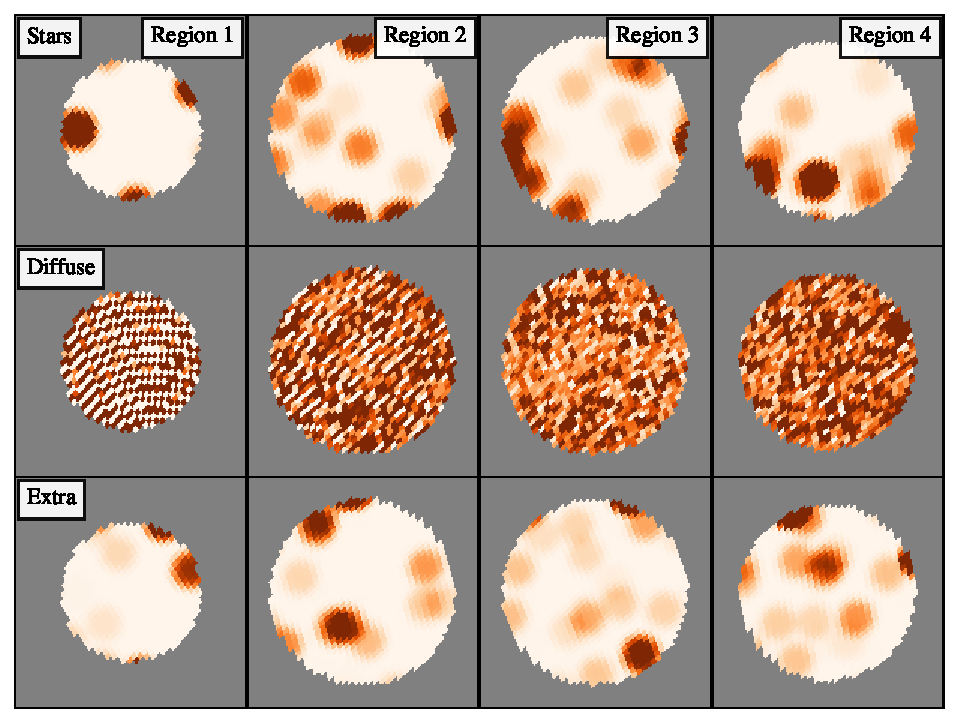
\includegraphics[width=\textwidth]{figs/regions/regions_01.pdf}\\
            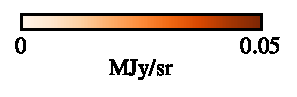
\includegraphics[width=0.3\textwidth]{figs/regions/cbar.pdf}\\

  \caption{The four regions from \cite{DIRBE2mass}, shown from left to right. From top to bottom, we have the star emission, the diffuse template and the extra sources.}
  \label{fig:regions}
\end{figure*}

The four regions are shown in Figure \ref{fig:regions}, left to right. We plot the stars, diffuse and extragalactic sources components for each region, showing the small scale structures. Differences in star classification between our analysis and \cite{DIRBE2mass} make it challenging to directly compare our amplitude estimates, but the sum of the bright and diffuse sources can still be compared. The Cosmoglobe analysis predicts about 20\% more total star emission, depending on the field and the frequency, which is probably due to having a much deeper star catalogue than 2MASS. By successfully modelling and removing more star emission, we are able to improve upon their limits on the CIB, as shown in \cite{CG02_02}. 

%\begin{figure}
%  \centering
%  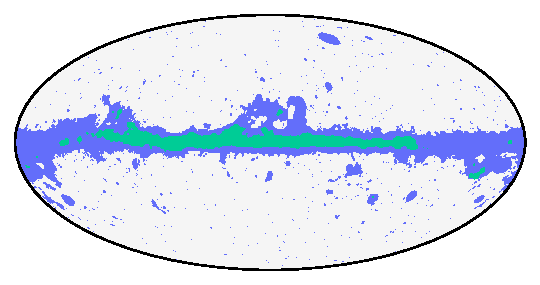
\includegraphics[width=\columnwidth]{figs/mask_proc_calib.pdf}
%  \caption{Processing masks use in the analysis.}
%  \label{fig:masks}
%\end{figure}

%Consistancy with WISE - maybe compare with a single WISE tile? I think the tile is probably too small for a useful comparison, and stitching together a mozaic is too complicated

\subsection{Extragalactic Sources?}
\label{sec:extragalactic?}

Throughout the paper, we have called this third class of bright sources that do not match against the PHOENIX database "Extra Sources", mostly as a easy placeholder name. Our processing is agnostic towards the properties of these sources, but we can investigate these sources by matching them against other datasets. One hypothesis we had about these sources is that they might be resolved extraglactic background sources, which would explain why the Gaia star parameters pipeline was unable to properly classify them.
 
To investigate this, we take the brightest 10 sources in the DIRBE 01 band, as well as 10 other randomly selected sources of the 66217 total extra sources, and look them up in the SIMBAD and VizieR query services, to try and get a sense of the classifications of these sources in other databases. The results are presented in table \ref{tab:exgal}.

\begin{table*}
    \centering
    \newcolumntype{C}{ @{}>{${}}r<{{}$}@{} }
    \begin{tabular}{l c c c c c c c}
    \hline
    \hline
     Src & $l$ & $b$ & $A_{01}$ & Mag$_{W1}$ & Closest Source ID & $\Delta r$ & Type \\ 
     & ($^{\circ}$) & ($^{\circ}$) & (MJy) & & & arcsec &  \\
    
     \hline
     1 \rule{0pt}{2ex} & 351.97 & 15.03 & 972 & 2.4 & Gaia DR2 6045630776564826368 & 0.06 & * \\
     2 & 199.84 & -8.94 & 725 & 1.35 & AllWISE	J055518.95+072220.3 & 0 & * \\
	 3 & 351.95 & 15.09 & 725 & 1.73 & hstID S8EN231745 & 0.03 & * \\
     4 & 272.65 & -39.30 & 619 & 3.16 & hstID S142070633 & 1.2 & -\\
	 5 & 35.50 & 27.83 & 601 & 1.73 & smssj 171432.09+142210.3 & 0.1 & *\\ 
	 6 & 199.81 & -8.99 & 548 & 3.61 & hstID N9I5116496 & 0.01 & *\\ 
	 7 & 35.57 &  27.80 & 513 & 0.57 & hstID N3VM068511 & 0.01 & * \\
	 8 & 199.79 & -8.96 & 495 & -1.38 & hstID N9I5116403 & 0.3 & * \\ 
	 9 & 272.69 & -39.30 & 495 & 5.01 & AllWISE	J043704.88-620608.5  & 0 & -\\ 
	 10 & 162.59 & 4.57 & 477 & 1.46 & hstID NCAJ155129 & 0.3 & *\\ 
	 11 & 126.12 & -6.72 & 0.81 & 4.29 & HD 236669 & 0.4 & Spectroscopic Binary\\ 
	 12 & 299.45 & 9.14 & 0.81 & 4.96 & HD 108499 & 0.1 & Spectroscopic Binary\\ 
	 13 & 68.98 & 2.35 & 7.2$\cdot 10^{-4}$ & 5.01 & IRAS 19534+3241 & 0.3 & Long-Period Variable\\
	 14 & 302.55 &  10.44 & 0.34 & 5.01 & IRAS 12461-5209 & 1.3 & Long Period Variable Candidate\\
	 15 & 56.88 & -4.15 & 0.46 & 4.40 & V* RW Sge  & 0.17 & Mira Variable \\
	 16 & 83.035 & 49.70 & 0.76 & 4.63 & HD 234253 & 0.4 & Star\\
	 17 & 5.02 & -1.36 & 8.1$\cdot 10^{-3}$ & 4.33 & IRAS 17592-2517 & 0.3 & Mira Variable\\ 
	 18 & 317.08 & -3.65 & 1.8 & 3.55 & IRAS 14569-6242 & 0.4 & Long period variable candidate \\
	 19 & 187.05 & -4.28 & 17.7 & -2.06 & V* Y Tau & 0.3 & Carbon Star\\
	 20 & 15.00 & 0.02 & 3.71 & 5.04 & 2MASS 18174772-1553381 & 0.38 & - \\
     \hline
    \end{tabular}
    \caption{Description of 20 extragalactic sources, the 10 brightest and 10 randomly selected ones. The bright sources are almost entirely found within the boundaries of other very bright sources in the optical (denoted with type *), so their brightnesses may be influenced by this confusion. Those with types listed as a dash have no catalogue information about their classifications.}
    \label{tab:exgal}
\end{table*}

The majority of the bright sources are within the saturation radii of other very bright sources in the optical, and so their lack of stellar parameters from Gaia (and potentially their large amplitudes) are likely related to confusion with the brighter nearby star. The ten dimmer objects are a range of irregular star types, which may also explain the lack of data from Gaia. Overall, it seems like 'Extragalactic Sources' is likely a misnomer, and this class of object is more likely to be poorly modelled stars within our own galaxy.

Gaia DR2 notes two limitations in their approach that may explain the makeup of these additional sources. Firstly, "All sources are treated as single stars," which could explain why so many binary objects are not fit successfully. Further down the list, they note that "...[in] crowded regions ... the integrated photometry is sometimes compromised ... As the two Gaia fields-of-view are projected onto a common focal plane, sources can overlap even in low density regions." \citep{gaiaClassification} This second limitation may explain the population of bright sources with no spectral data that are found within very bright objects and clusters.

\subsection{Beam Estimation}

Another comparison that can be taken between this work and other analyses is an assessment of the averaged beam profile. DIRBE measured their beams from the sky, although using only a small subset of the total dataset, so it is interesting to see if using the entire map can obtain similar or improved results.

To obtain an estimate of the beams directly from the data, we employ the following procedure in the star dominated channels. For a given frequency map at a band i, we can approximate the full data model as 

\begin{equation}
M_i \approx \sum_{n=1}^{N} p_n \circledast B_i,
\label{eq:beammodel}
\end{equation}

where $M$ is the map, $p_n$ are the list of all pointsources and $B$ is the beam window function. Equation \ref{eq:beammodel} is obviously not true in general, but for bands where the sky is dominated by pointsources this approach is at least approximately correct. If we take the zodi-subtracted maps and mask out the regions in the galactic center where we have known residuals from other components, then we have 

\begin{equation}
m \cdot M_i = \sum_{n=1}^{N} (m \cdot p_n) \circledast B_i,
\label{eq:maskedbeam}
\end{equation}

where $m$ is now a mask which removes the regions in the galactic center. In bands 1-4, where the point sources are by far the brightest signal, this assumption is enough to produce an estimate of the beam function by simply taking the expression and converting to $a_{l,m}$s such that for a single frequency

\begin{equation}
M'_{alm} = s'_{alm} \cdot B_{alm},
\label{eq:maskedbeam}
\end{equation}

where $M'$ is the masked map, and $s'$ is the masked sky, which is the sum of all the pointsources of equation \ref{eq:maskedbeam}. From here, it is a simple matter to divide the two quantities and convert to $C_l$s to extract the averaged beam window function $B_l$.

\begin{figure*}
  \centering
  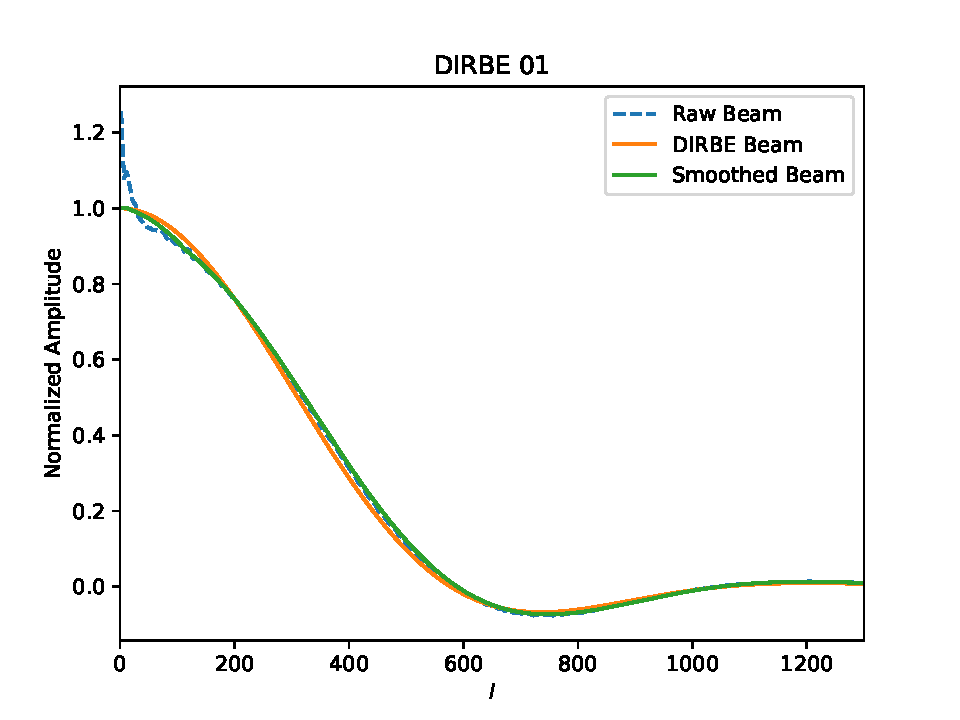
\includegraphics[width=0.49\textwidth]{figs/stacking/beam_01.pdf}
  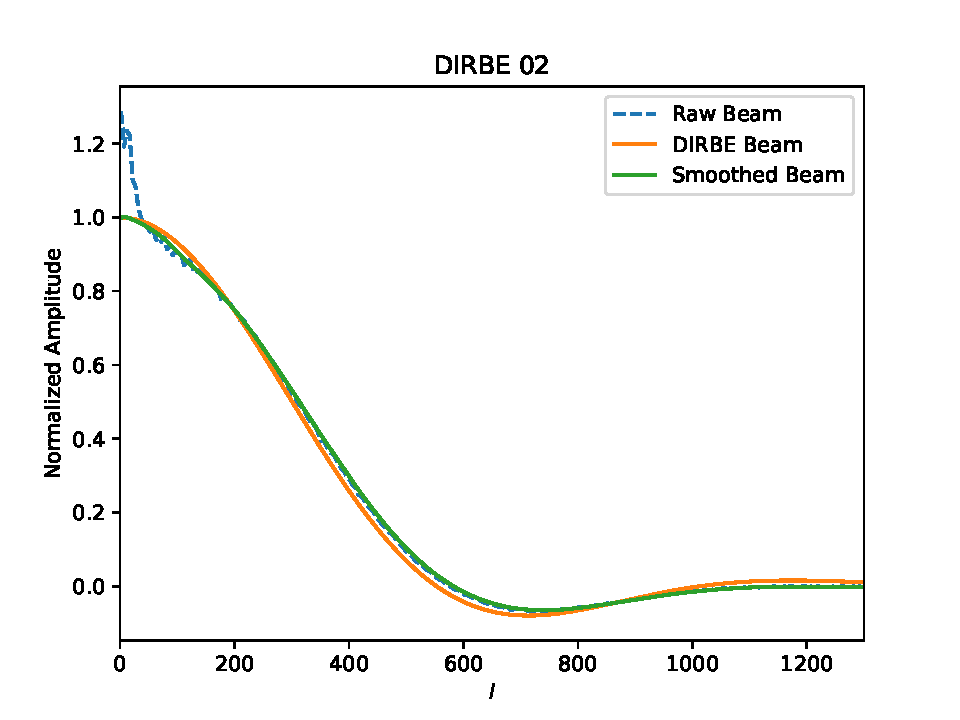
\includegraphics[width=0.49\textwidth]{figs/stacking/beam_02.pdf}\\
  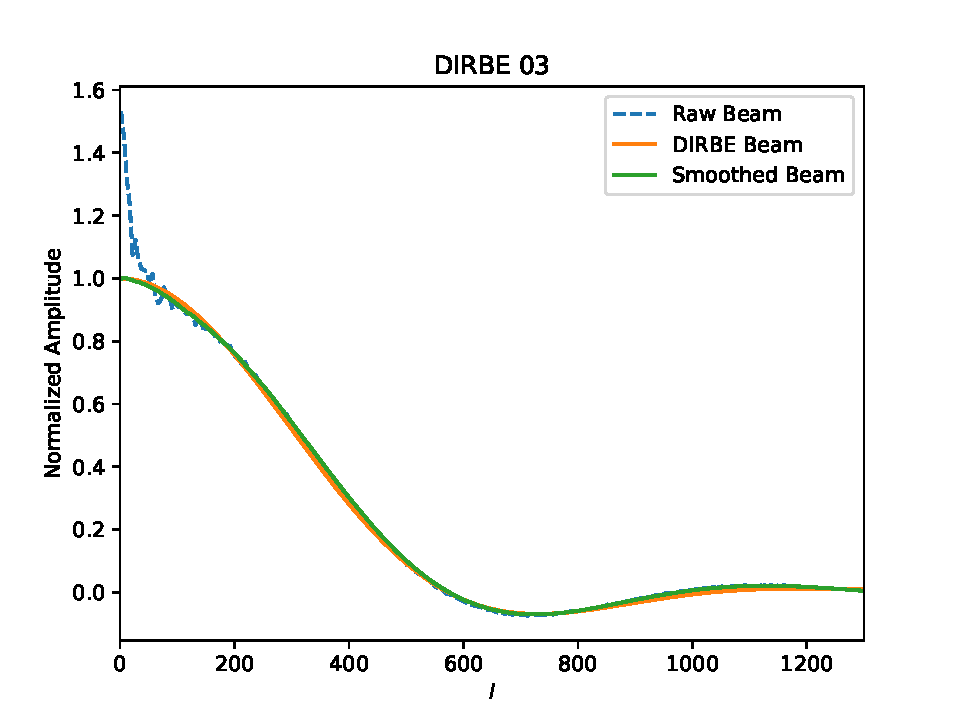
\includegraphics[width=0.49\textwidth]{figs/stacking/beam_03.pdf}
  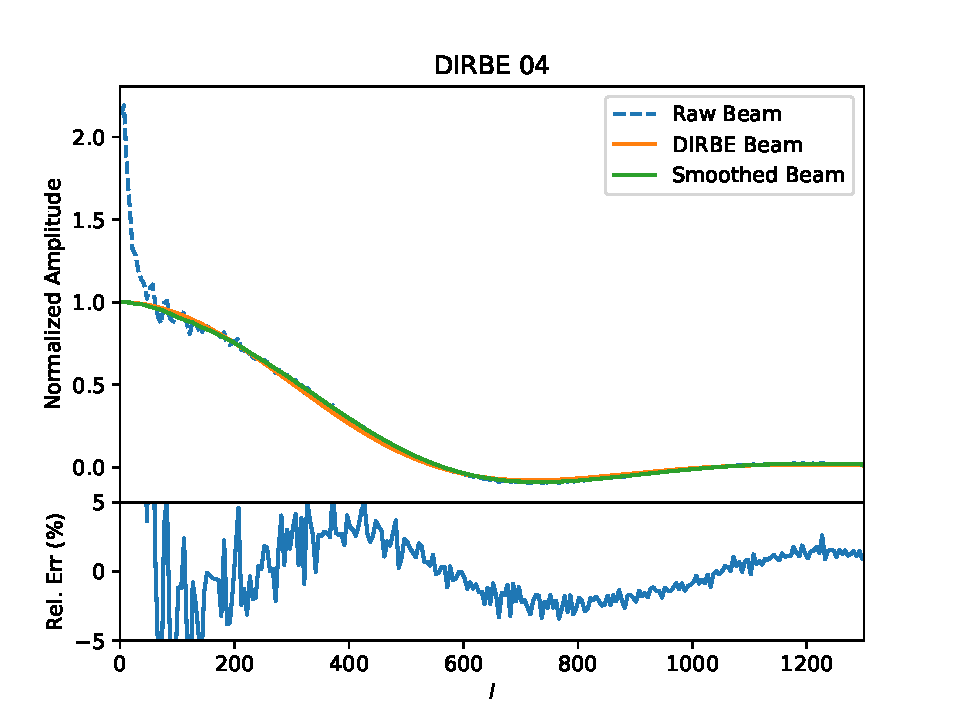
\includegraphics[width=0.49\textwidth]{figs/stacking/beam_04.pdf}\\

  \caption{Normalized beam estimates from pointsources in the first 4 DIRBE bands (blue), and the smoothed profile generated by masking the excess power at low $l$. Overplotted in orange are the $B_l$ profiles from the original DIRBE analysis for comparison.}
  \label{fig:beams}
\end{figure*}

In practise, doing the naive division of eq. \ref{eq:maskedbeam} results in a spectra that is dominated by poorly constrained multipoles. Instead, we can compute the binned quantity

\begin{equation}
\sum \limits_{l\ \mathrm{ bins}}\frac{\sum \limits_{l,m} M' s'}{\sum \limits_{l,m} s^{'2}}
\end{equation}

where we have dropped the subscript alm, and are summing the spectra over bins with width 5 in $l$. This has the advantage of reducing the noise in the beam estimate considerably by ensuring all bins contain non-zero denominators. Figure \ref{fig:beams} shows these window functions for bands 1-4. At low multipoles, it is clear that there is some additional contribution to the map which ends up in our beam estimates, most likely residual zodiacal light or other large scale leakage from other sky components. The dashed blue line shows the raw calculation, and the solid green line shows a smoothed extrapolation that removes this excess power. The curve is normalized to minimize the difference with the official DIRBE beam profiles (overplotted in orange).

The reconstructed beams are slightly wider than the profiles provided by the original DIRBE team, and do not exhibit as large of a negative dip in the $l=600-1000$ range, especially in the DIRBE 02 channel at 2.2 $\mu$m. Comparing templates of pointsources made with these two beams, we find differences on the order of $10^{-14}$ MJy/sr, which is negligible at these wavelengths, so we can conclude that our approach reproduced the DIRBE beams with high fidelity, and could be an interesting way to estimate beam profiles in other experiments at the frequencies.

\section{Conclusions}
\label{sec:conclusions}

Stars are a critical component of the infrared sky, which must be correctly modelled in order to avoid contaminating other components. 

Figure \ref{fig:sed} shows the full sky average star SED derived from this work, plotted with the other sky signals as a function of frequency and wavelength, from the radio all the way to the infrared. The Cosmoglobe DR2 release, which this paper forms part of, is the first time a unified model of the sky has been shown to successfully describe all these frequencies, and the star model presented here is an integral part of this work.

\begin{figure*}
  \centering
  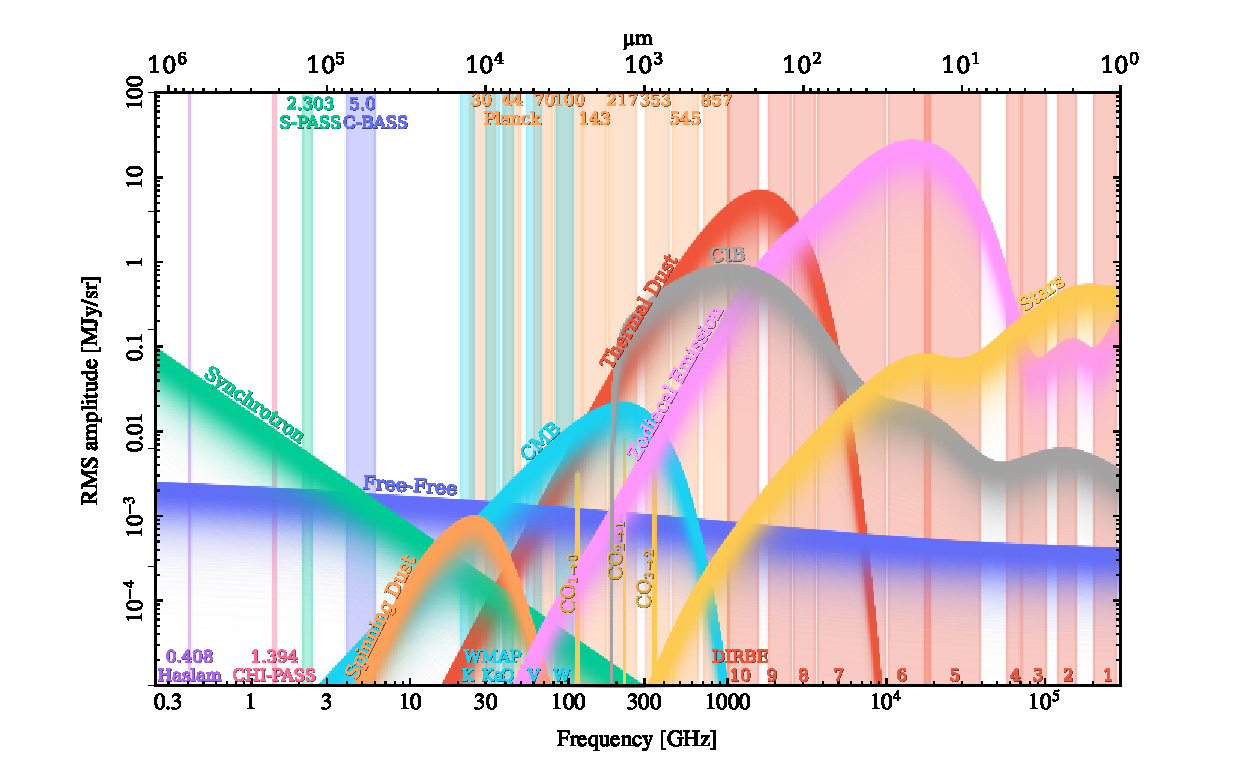
\includegraphics[width=1.1\textwidth]{figs/sed/cg_spec.pdf}
  \caption{Components of the infrared temperature sky from 0.1$\mu$m to 1m wavelengths. The approximate contribution from stars is shown in yellow, and the observing bands from various experiments are indicated by the vertical lines. TODO:The splines for zodi and stars are a mess, I need to fix them still}
  \label{fig:sed}
\end{figure*}

Using the three classes of sources described in this paper, we were able to model 98\% of the observed DIRBE flux density at 1.25$\mu$m, dropping to 3\% at 25$\mu$m. Despite some evidence of internal degeneracies caused by excess parameters, the star model showed robust mixing, and was able to fully describe the summed star emission in an effective manner. Our model was able to characterize and remove more star emission than previous works, which consequently was able to produce lower residuals and better constraints on the CIB monopoles, as discussed in the companion paper \citet{CG02_03}. Stars form the dominant foreground at these wavelengths, and so this model is an important contribution to the overall Cosmoglobe sky model, and can be re-used and adapted for future analyses using that framework.

\subsection{Future Work}

Including additional high frequency data directly in the the full run would be an important next step for this work, and will be the subject of future exploration in the collaboration. WISE is a major candidate experiment here, but also   AKARI \citep{akari} and IRAS \citep{iras} would be important complements to the work performed here. Incorporating these data directly could potentially give enough extra information to constrain the star SEDs directly instead of pre-computing them.

Additionally, the star model could be improved by the inclusion of a dust extinction term. This could be achieved by adding a dust-correlated template map with a negative amplitude, that corresponds to absorption, and fit the amplitude and spectral behaviours of that component as well.

Another place within the model where there is room for improvement is in the treatment of the beams. Instead of assuming spherically symmerized beams, we could properly treat the unique square shape of the DIRBE response function, using techniques like deconvolution mapmaking \citep{artdeco}.

Finally, we could also improve our handling of the brightest stars, determining more accurate SEDs for those with $T_{\mathrm{eff}}>12000$K. This may help reduce the residuals around the brightest sources, and, combined with pruning the bright sources with 0 amplitudes could reduce the overall residual levels around these bright sources.


\begin{acknowledgements}
 The current work has received funding from the European
  Union’s Horizon 2020 research and innovation programme under grant
  agreement numbers 819478 (ERC; \textsc{Cosmoglobe}) and 772253 (ERC;
  \textsc{bits2cosmology}). Some of the results in this paper have been derived using the HEALPix \citep{healpix} package.
  We acknowledge the use of the Legacy Archive for Microwave Background Data
  Analysis (LAMBDA), part of the High Energy Astrophysics Science Archive Center
  (HEASARC). HEASARC/LAMBDA is a service of the Astrophysics Science Division at
  the NASA Goddard Space Flight Center.  
  
   This publication makes use of data products from the Wide-field Infrared Survey Explorer, which is a joint project of the University of California, Los Angeles, and the Jet Propulsion Laboratory/California Institute of Technology, and NEOWISE, which is a project of the Jet Propulsion Laboratory/California Institute of Technology. WISE and NEOWISE are funded by the National Aeronautics and Space Administration.
   
   This work has made use of data from the European Space Agency (ESA) mission
{\it Gaia} (\url{https://www.cosmos.esa.int/gaia}), processed by the {\it Gaia}
Data Processing and Analysis Consortium (DPAC,
\url{https://www.cosmos.esa.int/web/gaia/dpac/consortium}). Funding for the DPAC
has been provided by national institutions, in particular the institutions
participating in the {\it Gaia} Multilateral Agreement.
\end{acknowledgements}


%-------------------------------------------------------------
%                                       Table with references 
%-------------------------------------------------------------
%

\bibliographystyle{aa}
\bibliography{references, ../../common/CG_bibliography}
\end{document}
%%%% End of aa.dem
